% Options for packages loaded elsewhere
\PassOptionsToPackage{unicode}{hyperref}
\PassOptionsToPackage{hyphens}{url}
%
\documentclass[
  11pt,
]{article}
\usepackage{amsmath,amssymb}
\usepackage{iftex}
\ifPDFTeX
  \usepackage[T1]{fontenc}
  \usepackage[utf8]{inputenc}
  \usepackage{textcomp} % provide euro and other symbols
\else % if luatex or xetex
  \usepackage{unicode-math} % this also loads fontspec
  \defaultfontfeatures{Scale=MatchLowercase}
  \defaultfontfeatures[\rmfamily]{Ligatures=TeX,Scale=1}
\fi
\usepackage[]{mathpazo}
\ifPDFTeX\else
  % xetex/luatex font selection
\fi
% Use upquote if available, for straight quotes in verbatim environments
\IfFileExists{upquote.sty}{\usepackage{upquote}}{}
\IfFileExists{microtype.sty}{% use microtype if available
  \usepackage[]{microtype}
  \UseMicrotypeSet[protrusion]{basicmath} % disable protrusion for tt fonts
}{}
\makeatletter
\@ifundefined{KOMAClassName}{% if non-KOMA class
  \IfFileExists{parskip.sty}{%
    \usepackage{parskip}
  }{% else
    \setlength{\parindent}{0pt}
    \setlength{\parskip}{6pt plus 2pt minus 1pt}}
}{% if KOMA class
  \KOMAoptions{parskip=half}}
\makeatother
\usepackage{xcolor}
\usepackage[margin=1in]{geometry}
\usepackage{graphicx}
\makeatletter
\def\maxwidth{\ifdim\Gin@nat@width>\linewidth\linewidth\else\Gin@nat@width\fi}
\def\maxheight{\ifdim\Gin@nat@height>\textheight\textheight\else\Gin@nat@height\fi}
\makeatother
% Scale images if necessary, so that they will not overflow the page
% margins by default, and it is still possible to overwrite the defaults
% using explicit options in \includegraphics[width, height, ...]{}
\setkeys{Gin}{width=\maxwidth,height=\maxheight,keepaspectratio}
% Set default figure placement to htbp
\makeatletter
\def\fps@figure{htbp}
\makeatother
\setlength{\emergencystretch}{3em} % prevent overfull lines
\providecommand{\tightlist}{%
  \setlength{\itemsep}{0pt}\setlength{\parskip}{0pt}}
\setcounter{secnumdepth}{-\maxdimen} % remove section numbering
\newlength{\cslhangindent}
\setlength{\cslhangindent}{1.5em}
\newlength{\csllabelwidth}
\setlength{\csllabelwidth}{3em}
\newlength{\cslentryspacingunit} % times entry-spacing
\setlength{\cslentryspacingunit}{\parskip}
\newenvironment{CSLReferences}[2] % #1 hanging-ident, #2 entry spacing
 {% don't indent paragraphs
  \setlength{\parindent}{0pt}
  % turn on hanging indent if param 1 is 1
  \ifodd #1
  \let\oldpar\par
  \def\par{\hangindent=\cslhangindent\oldpar}
  \fi
  % set entry spacing
  \setlength{\parskip}{#2\cslentryspacingunit}
 }%
 {}
\usepackage{calc}
\newcommand{\CSLBlock}[1]{#1\hfill\break}
\newcommand{\CSLLeftMargin}[1]{\parbox[t]{\csllabelwidth}{#1}}
\newcommand{\CSLRightInline}[1]{\parbox[t]{\linewidth - \csllabelwidth}{#1}\break}
\newcommand{\CSLIndent}[1]{\hspace{\cslhangindent}#1}
\usepackage{float} \usepackage{array} \usepackage{longtable} \usepackage{caption} \usepackage{booktabs}
\usepackage{booktabs}
\usepackage{longtable}
\usepackage{array}
\usepackage{multirow}
\usepackage{wrapfig}
\usepackage{float}
\usepackage{colortbl}
\usepackage{pdflscape}
\usepackage{tabu}
\usepackage{threeparttable}
\usepackage{threeparttablex}
\usepackage[normalem]{ulem}
\usepackage{makecell}
\usepackage{xcolor}
\ifLuaTeX
  \usepackage{selnolig}  % disable illegal ligatures
\fi
\IfFileExists{bookmark.sty}{\usepackage{bookmark}}{\usepackage{hyperref}}
\IfFileExists{xurl.sty}{\usepackage{xurl}}{} % add URL line breaks if available
\urlstyle{same}
\hypersetup{
  pdfauthor={Nicolas Restrepo Ochoa; Turgut Keskintürk},
  hidelinks,
  pdfcreator={LaTeX via pandoc}}

\title{Measuring Movement in Cultural Landscapes\footnote{We thank
  Stephen Vaisey, Tom Wolff, Andrés Castro Araújo, the participants of
  Worldview Lab at Duke University and Cultural Evolution Lab at
  University of California at Davis for their helpful comments. The
  replication files for the article can be found at
  github.com/NicolasRestrep/landscapes.}}
\author{Nicolas Restrepo Ochoa\footnote{Department of Anthropology,
  University of California, Davis.} \and Turgut Keskintürk\footnote{Department
  of Sociology, Duke University.}}
\date{October 11, 2023}

\begin{document}
\maketitle
\begin{abstract}
Culture is often conceptualized as a \emph{landscape}, where the peaks
represent popular beliefs, institutions or practices, while the valleys
represent those that receive infrequent attention. In this article, we
build on this metaphor, and explore how individuals navigate these
cultural landscapes. Using longitudinal data from the National Study of
Youth and Religion, we follow participants' survey response trajectories
across three cultural domains, each with particular topographical
features. We show that movement across cultural landscapes is adequately
captured by a gravitational model of change, which specifies transition
probabilities among cultural positions as a function of the distance
between them and how populated they are. Nonetheless, the kind of
movement that such a gravitational model would predict varies widely
depending on the initial topography of the landscape. Our work
highlights that charting landscapes is not only useful cartography, but
also an analytical tool that helps us understand the kind of cultural
trajectories we should expect individuals to follow.
\end{abstract}

\hypertarget{introduction}{%
\section{Introduction}\label{introduction}}

One widespread metaphor to think about culture is to conceptualize it as
a ``landscape,'' where certain cultural objects --personal beliefs,
daily practices, or institutional structures-- are closer to some than
others. We intuitively know that various positions within those
landscapes are highly prevalent: despite their many differences, moral
discourses or religious doctrines, across history and social groups,
share certain features. We recognize, for instance, that most such
doctrines have proscriptions against murder and theft, but fewer against
the consumption of animals with cloven hooves. Hence, the landscape
metaphor is somewhat literal: once we examine a given cultural space, we
recognize the shared features that make certain positions close to one
another, and we can tell that there are populated areas and relatively
sparse regions.

In this article, we build on this metaphor and explore \emph{personal
culture} -- the bits of culture that are manifest in individual beliefs,
attitudes, and preferences (Lizardo 2017). We propose an approach to
formalizing cultural landscapes using survey data, and argue that this
approach is useful for understanding how personal culture is organized.
Moreover, we argue that the landscape metaphor is not just useful
cartography, but also an analytical tool to explore individual cultural
movement.

Using panel data from the National Study of Youth and Religion (NSYR)
and simulation studies, we ask whether the organization of cultural
landscapes predicts cultural trajectories. We show that cultural
landscapes allow us to understand the dynamism of cultural change:
people's probability to change or remain stable varies according to the
organization of the landscape. We argue that knowing how people are
distributed within cultural positions is informative to predict
subsequent states, as some distributions make particular trajectories
more or less likely.

The article is structured as follows. We begin by reviewing several
common threads within the interdisciplinary efforts to represent culture
as a landscape. In the second section, we conceptualize trajectories
across cultural landscapes as a Markovian process, where each position
in the landscape is associated with a set of transition probabilities.
This allows us to specify several generative models of cultural change.
We test these models against the empirical data from the NSYR and use
simulations to emphasize that these models imply different trajectories
depending on the initial topography of the space. We conclude by
examining the implications of this exercise, emphasizing the resonance
with ideas of duality in cultural sociology.

\hypertarget{understanding-culture-as-landscape}{%
\section{Understanding Culture as
Landscape}\label{understanding-culture-as-landscape}}

\hypertarget{an-approach-for-cartography}{%
\subsection{An Approach for
Cartography}\label{an-approach-for-cartography}}

The metaphor of culture as landscape is widespread across scientific
disciplines, the general idea being that cultural objects, whether they
are writing instruments or religions, are defined through the parameters
of an underlying landscape (Poulsen and DeDeo 2023a, 2023b). The first
of these parameters is \emph{cardinality}, i.e., the set of total
positions within the cultural landscape. The positions are represented
as binary strings that denote the presence or absence of certain
cultural features -- e.g., 1 for having feature X and 0 for not having
feature X. Cardinality allows us to understand the relationships among
cultural objects in terms of proximity and distance: fountain pens are
somewhat closer to ballpoint pens than they are to chalk, and
Zoroastrianism is closer to Christianity than to Buddhism. The second
parameter of interest is \emph{topography}, i.e., the relative height of
each position in relation to others. This means that a landscape has
some volume, determined either by something's perceived utility (you
would probably rather take notes with a pencil than charcoal), or mere
occupancy (Christianity has currently more adherents in the world than
Zoroastrianism).

The popularity of this metaphor is partly because it is useful for
understanding several biological and social phenomena. For researchers
interested in evolutionary dynamics, the landscape metaphor points
towards where potential attractors --i.e., high points in the
landscape-- might lie (Falandays and Smaldino 2021), an example being
the relatively low number of positions occupied within the set of all
potential positions in the history of world religions (Norenzayan 2013;
Poulsen and DeDeo 2023a).\footnote{In other words, given the almost
  infinite combination of features a religion could have, it is quite
  striking that most look broadly similar. Most religions, then, are
  concentrated in a relatively small area of the cultural landscape.} In
studies of social structure, understanding the relationship between
individual actors and the positions they occupy in a given cultural
landscape is essential (Mark 1998; Martin and Desmond 2010). Several
important insights from the sociological study of culture have come from
the deceptively simple idea that people who occupy proximate positions
in cultural landscapes tend to share other social characteristics as
well (Baldassarri and Goldberg 2014; Bonikowski and DiMaggio 2016;
DellaPosta, Shi, and Macy 2015; Goldberg 2011).

It is relatively straightforward to formalize these ideas. One strategy
is to use binary strings of length \(n\), where \(n\) refers to the size
of elements that constitute the given cultural system. We can use these
strings to outline the positions that make up the cultural landscapes
(Poulsen and DeDeo 2023a, 2023b). Going back to the example of religion,
we might think about different elements that describe the cultural
system of a religion: the institution of monotheism, the belief in an
afterlife, or practices of dietary restrictions. The number of these
elements would be equal to the length of a string, and the presence or
absence of such elements would be denoted by 1s and 0s, respectively.
Hence, if we were to characterize Christianity based on the three
features just selected, it would occupy the position C = {[}1, 1, 1{]}
in a three-dimensional space, and this position would imply that all
features within the landscape exist in the cultural position of
Christianity.

This basic algebraic representation is highly useful, and we can define
cardinality and topography easily. In this three-dimensional landscape,
the total set of positions would be defined as \(2^3 = 8\). Thus, in the
general case, the number of elements \(n\) can be mapped to \(2^n\).
Moving from this, we can define the total distance between positions as
the absolute value of the Hamming distance between each string of
possible cultural positions, calculated as

\[
D_{p_1, p_2} = | p_1 - p_2 |
\]

Cultural positions that are one step away from each other --e.g.,
\([1, 1, 1]\) and \([1, 1, 0]\)-- are considered to be adjacent. We can
then represent these positions in a graph, where each vertex represents
a position in the landscape, and the edges between vertices capture the
adjacency between them. The left panel in Figure 1 depicts the cube
emerging from this three-dimensional example.

\begin{figure}[htp]
\begin{center}
\caption*{Figure 1: Cubes from Three-Dimensional Landscape}

\begin{center}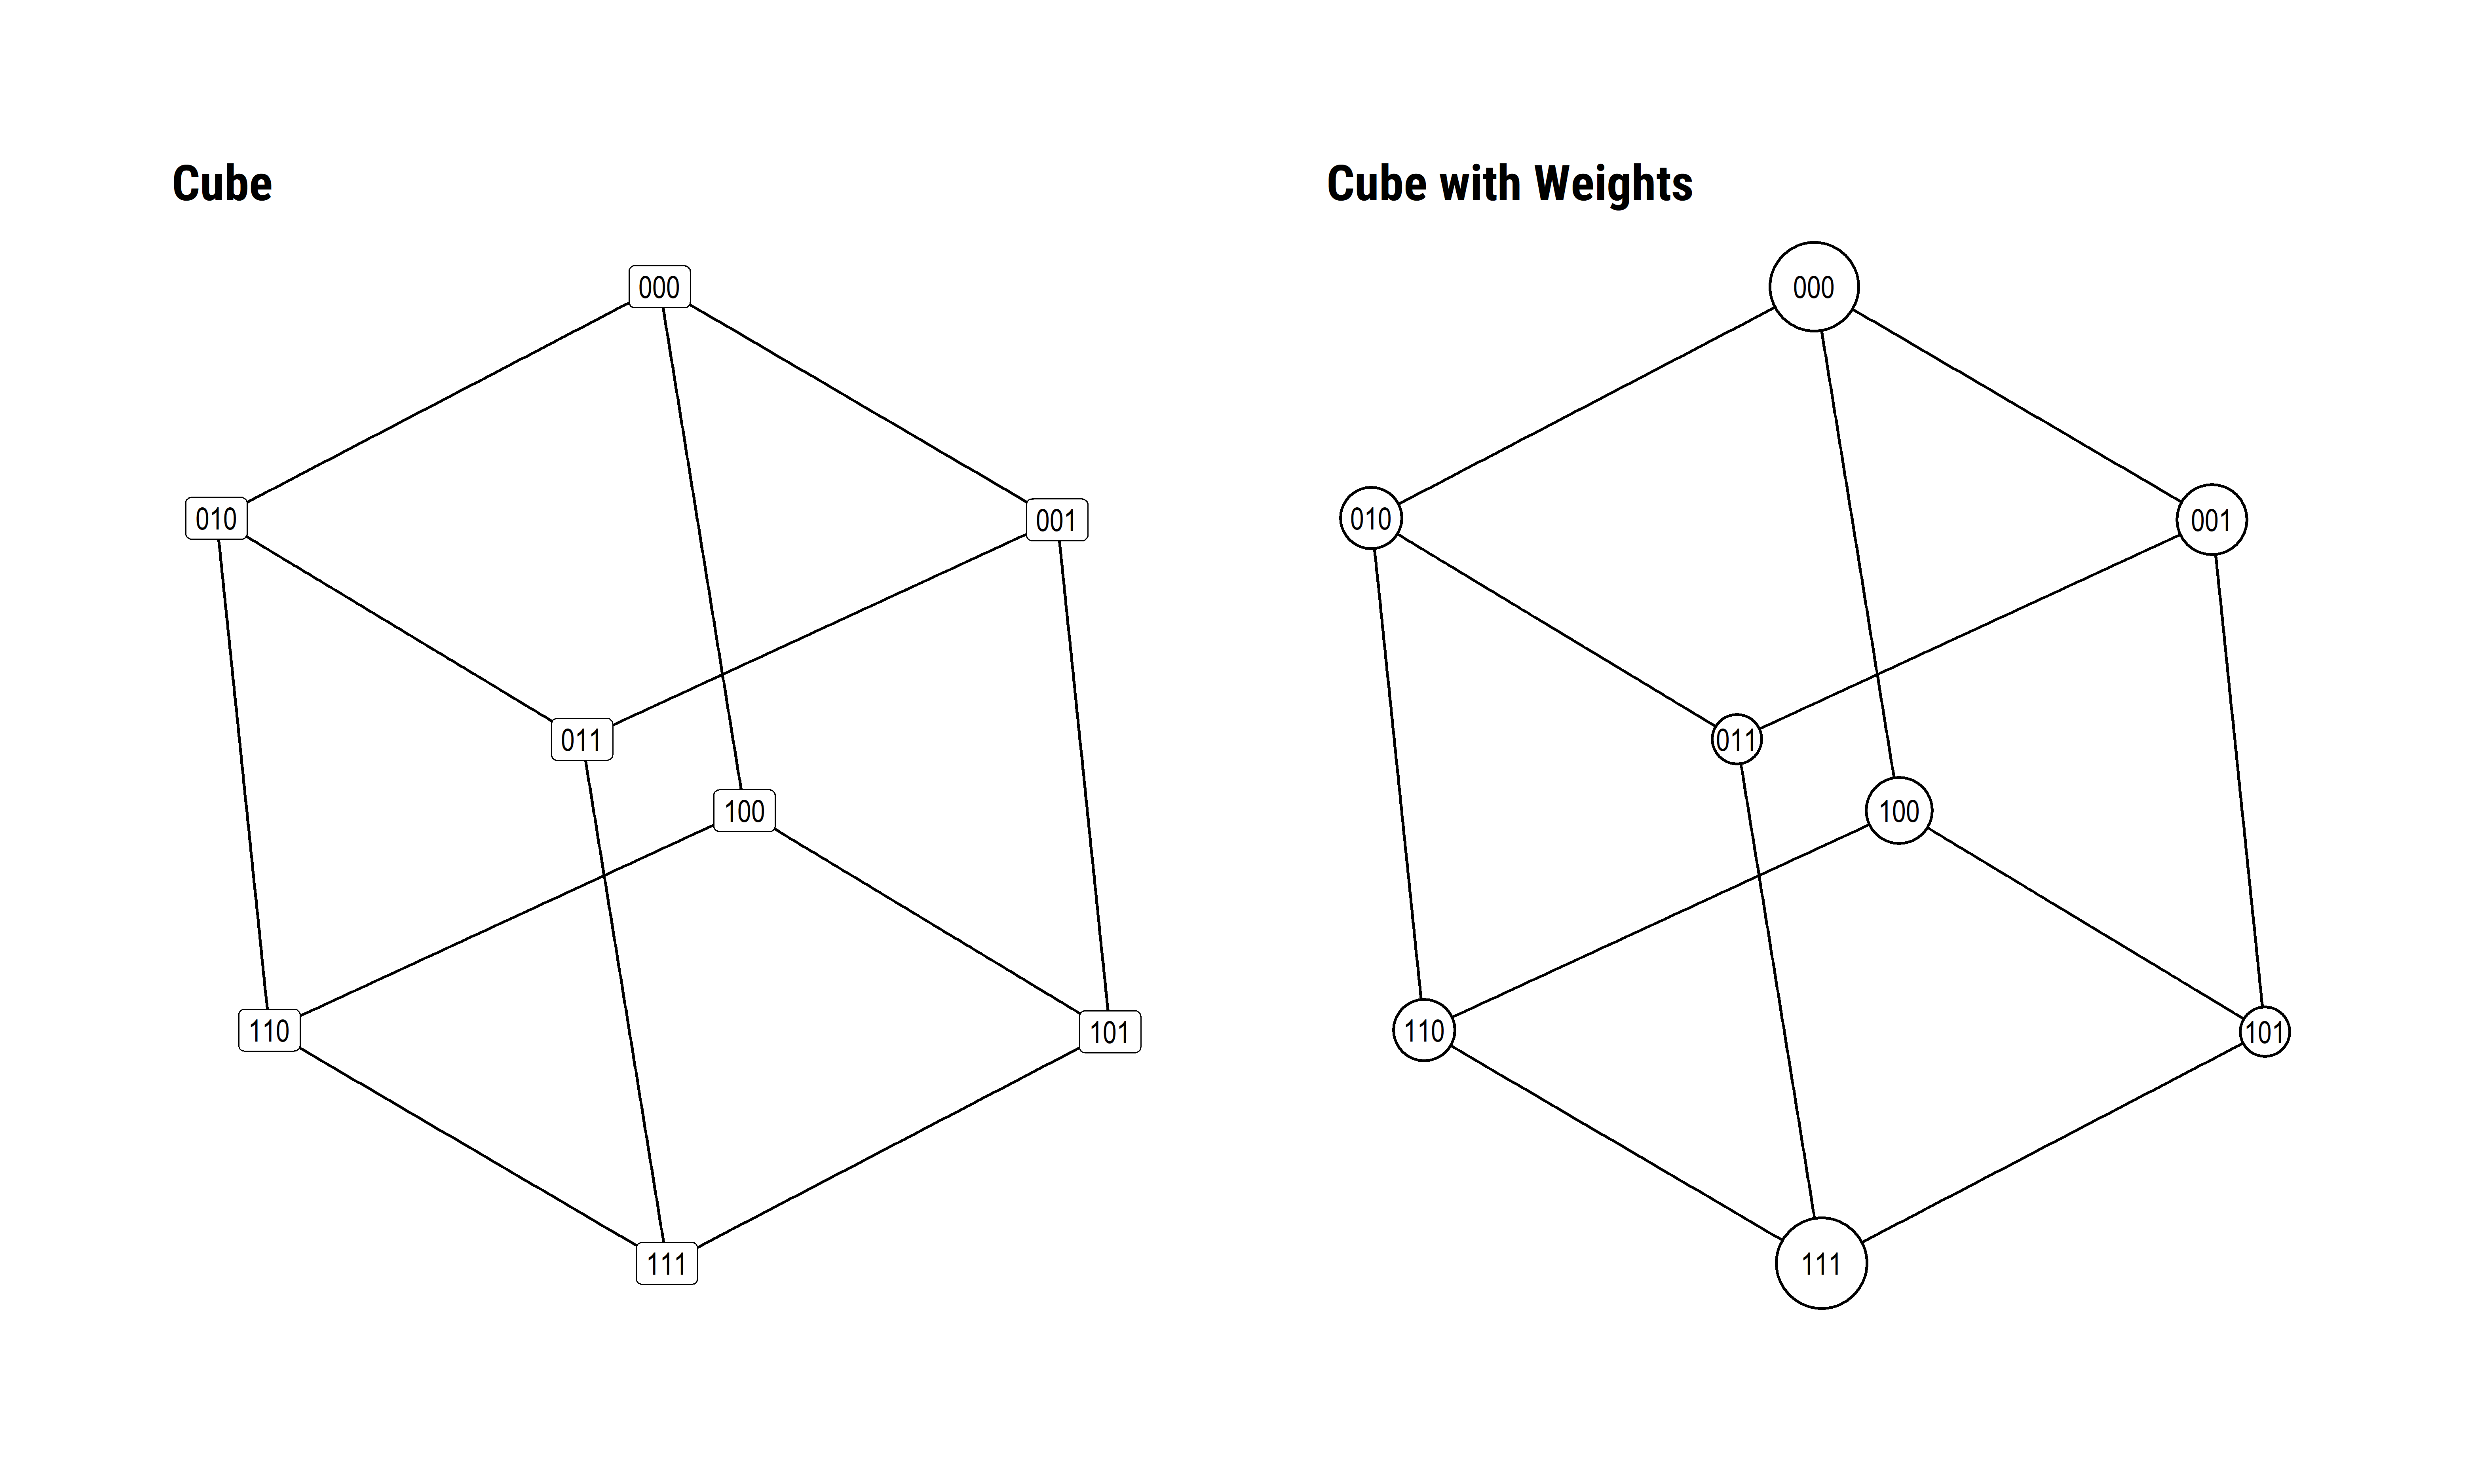
\includegraphics[width=1\linewidth]{../figures/figure_1} \end{center}

\end{center}
\end{figure}

Having defined the \emph{cardinality} of a landscape, how many positions
there are and how they are placed in relation to each other, we can also
examine its \emph{topography}. This means the landscape is not flat, but
rather has volume. The most famous model for generating these binary
representations with unit volumes is called an NK Model (Kauffman and
Weinberger 1989). In these models, the central parameter is
\emph{ruggedness}, i.e., the correlation between the heights of adjacent
positions. A landscape with minimal ruggedness implies that height
across positions increases or decreases in expected ways, and the height
of one's current position is quite predictive of what one might expect
in adjacent spots. In a maximally rugged landscape, however, the height
between positions is relatively unrelated, and one step might lead to a
giant increase or a sharp drop. The topography of the landscape is this
highly important because it affects how actors or groups navigate it. In
spaces with minimal ruggedness, we expect there to be one global peak,
and simply walking towards the highest adjacent position is a good
strategy to reach that peak. In a rugged landscape, though, such a
strategy would likely lead us to be stuck in a local optima. The
metaphor of culture as a landscape, then, owes part of its usefulness to
being able to capture these dynamics.

\hypertarget{the-social-organization-of-personal-culture}{%
\subsection{The Social Organization of Personal
Culture}\label{the-social-organization-of-personal-culture}}

Studies of ``personal culture,'' culture manifest in attitudes, beliefs,
and preferences (Lizardo 2017), have also drawn heavily from the culture
as a landscape metaphor. This is perhaps most apparent in the argument
that individual differences in personal culture can be captured in an
\(n\)-dimensional ``belief space'' (Martin 2000), much like the religion
landscape above. One consistent observation within this literature is
that actors' positions generally overlap: we often observe clusters of
individuals who share similar positions within the overall belief space
(Boutyline 2022; Goldberg 2011; Hunzaker and Valentino 2019). Hence,
this approach relates individual respondents with positions that have
certain frequencies at the group level, where we have a space of
positions --\emph{cardinality}-- that are more or less proximate to each
other, and that are more or less occupied --\emph{topography}. Tracing
such landscapes helps us understand the organization of personal
culture: to see how individuals are distributed across positions, and
what regions are more populated.

One underlying principle that governs these various research streams is
the notion of \emph{duality}, the idea that actors are defined through
groups and groups are defined through actors. Suppose that a landscape
consists of various identifiable positions that index the presence or
absence of cultural beliefs or institutions. Breiger (1974) states that
we can use this basic structure to extract two kinds of information: one
of ``actor-to-actor'' relations and one of ``group-to-group'' relations.
As actors cluster around similar regions, to the extent that they share
similar cultural positions, we can draw two insights. First, we learn
about what kinds of actors end up connected by sharing a cultural
position. Second, we can examine the kind of cultural positions that go
together because they share the same occupants. Similar to the culture
as landscape approach, the principle of duality attempts an
understanding of the structure of a given cultural domain.\footnote{We
  can follow the thread on Christianity and Zoroastrianism once more:
  the principle of duality says that the extent to which these two
  traditions share certain attributes defines how close they are, while
  we understand the connections between these same attributes as the
  number of shared ties they possess in the overall landscape.
  Sociologists exploited these ideas in several ways, most notably by
  conceptualizing belief systems as the co-occurrence of cultural
  positions (Boutyline and Vaisey 2017) or positions in a set of
  potential ordered pairs (Wiley and Martin 1999).}

Yet, what does this landscape do? The principle of duality is often used
to understand \emph{cultural cartographies}, though the organization of
culture might, at least in principle, provide information about
\emph{cultural movement}. As Martin (2000) emphasized before, a picture
from a low-orbiting satellite would give us the map, but also help us
figure out where the roads are. After all, people live through time,
either reproducing or changing the organization of the landscapes. If
duality is indeed the underlying principle, these cartographies might
not just help us see what culture is like, they might also store
``information about {[}potential{]} paths that {[}people will{]} take''
(Lee and Martin 2018:19), or what culture \emph{will} be like. In the
next section, we follow this reasoning and formalize a Markovian model
of cultural movement in longitudinal data.

\hypertarget{a-markovian-model-of-cultural-movement}{%
\section{A Markovian Model of Cultural
Movement}\label{a-markovian-model-of-cultural-movement}}

We propose that the organization of a cultural landscape --i.e., the
distribution of cultural positions and the emergent topography at time
\(t\)-- is instrumental to understanding one's cultural trajectory. This
trajectory can easily be formalized as a Markov process, where a
landscape changes from one state to another. This is effectively an
\emph{accounting} of transitions: we observe the number of people
occupying a position at each time point, and analyze the movements
--say, from position \([1,1,1]\) to position \([1,1,0]\)-- within and
between landscape positions. Each of these movements is associated with
a transition probability; when put together, these probabilities
constitute a transition matrix that provides information about the
future states of the distribution. With this framework, we can examine
whether actors tend to stay put in their initial positions, hover around
adjacent locations, or make long-distance jumps within a period of time.

Let us go through an example, and follow a three-feature landscape, like
the one we saw above. We have two pieces of information in this
Markovian system, the first of which describes the state at \(t_0\). In
this case, this is a vector \(w\) of equal length to the number of
positions that constitute the landscape -- each of these positions is
occupied by actors.\footnote{Remember that (a) each feature is defined
  with presence (1s) and absence (0s), and (b) since there are 3 unique
  slots, we have \(2^3 = 8\) unique positions.} The second is the matrix
of transitions, which stipulates how likely certain movements are among
these positions. Imagine that, in its initial state at \(t_0\), this is
a landscape with two high peaks at {[}1,1,1{]} and {[}0,0,0{]}, with all
the other positions only sparsely populated. Our vector of weights \(w\)
in this hypothetical case would be:

\[
w_0 = (13,5,3,2,4,2,3,14)
\]

The right panel of Figure 1 shows this landscape, where the size of the
vertices (i.e., the positions) is equal to the number of cultural units
(captured in \(w_0\)) occupying those positions.

Now that we described the landscape, let us imagine that this is a
completely stationary system, such that all actors will stay in their
positions from one time point to the next. The transition matrix \(T\),
in this example, will be an \(N \times N\) matrix, where \(N\) is the
number of unique positions. Given the system is stationary, this matrix
contains 1s in the diagonal and 0s everywhere else:

\[
T_{8,8} =
\begin{pmatrix}
1 & 0 & 0 & 0 & 0 & 0 & 0 & 0  \\
0 & 1 & 0 & 0 & 0 & 0 & 0 & 0  \\
0 & 0 & 1 & 0 & 0 & 0 & 0 & 0  \\
0 & 0 & 0 & 1 & 0 & 0 & 0 & 0  \\
0 & 0 & 0 & 0 & 1 & 0 & 0 & 0  \\
0 & 0 & 0 & 0 & 0 & 1 & 0 & 0  \\
0 & 0 & 0 & 0 & 0 & 0 & 1 & 0  \\
0 & 0 & 0 & 0 & 0 & 0 & 0 & 1 
\end{pmatrix}
\]

In this system, actors will stay in their positions from one time point
to another, and, therefore, have 0 probability of moving anywhere else.
In this transition matrix, \(T_{i,j}\) represents the probability of
moving from position \(i\) to position \(j\). In our example, an
individual located in any given position has 8 possible moves: they can
either stay put, or move to the other seven positions. Each of those 8
moves will have a probability associated with it, and these will be
encoded in the row associated with the position where the actor is
located at time \(t\). Given that our system is fully stationary, all
probability is concentrated in the diagonal, so we know individuals will
stay put.

The transition matrix \(T\) gives us one generative model that makes
particular predictions about how a cultural landscape should change over
time. In the example above, we know with certainty what every actor in
the system will do. Hence, we can perfectly predict what the system will
look like in a future time-step. In other words, there is only one
realization at any future time point that is consistent with that
transition matrix: everyone stays where they are. If we take the same
initial occupancy weights at \(w_0\) as above, the realization matrix
for this model would look like this:

\[
R_{8,8} =
\begin{pmatrix}
13 & 0 & 0 & 0 & 0 & 0 & 0 & 0  \\
0 & 5 & 0 & 0 & 0 & 0 & 0 & 0   \\
0 & 0 & 3 & 0 & 0 & 0 & 0 & 0   \\
0 & 0 & 0 & 2 & 0 & 0 & 0 & 0   \\
0 & 0 & 0 & 0 & 4 & 0 & 0 & 0   \\
0 & 0 & 0 & 0 & 0 & 2 & 0 & 0   \\
0 & 0 & 0 & 0 & 0 & 0 & 3 & 0   \\
0 & 0 & 0 & 0 & 0 & 0 & 0 & 14 
\end{pmatrix}
\]

Now, let's consider another model, where all movements between any two
positions are equally probable. The transition matrix for this random
model would look like this:

\[
T_{8,8} =
\begin{pmatrix}
\frac{1}{8} & ... & ... & ... & ... & ... & ... & \frac{1}{8}           \\
\frac{1}{8} & \frac{1}{8} & ... & ... & ... & ... & ... & \frac{1}{8}   \\
\frac{1}{8} & ... & \frac{1}{8} & ... & ... & ... & ... & \frac{1}{8}   \\
\frac{1}{8} & ... & ... & \frac{1}{8} & ... & ... & ... & \frac{1}{8}   \\
\frac{1}{8} & ... & ... & ... & \frac{1}{8} & ... & ... & \frac{1}{8}   \\
\frac{1}{8} & ... & ... & ... & ... & \frac{1}{8} & ... & \frac{1}{8}   \\
\frac{1}{8} & ... & ... & ... & ... & ... & \frac{1}{8} & \frac{1}{8}   \\
\frac{1}{8} & ... & ... & ... & ... & ... & ... & \frac{1}{8} 
\end{pmatrix}
\]

In this case, we can think of each row as representing a fairly weighted
8-sided die. We roll the die as many times as there are occupants in the
corresponding position at \(t_0\), and record the new positions. For
instance, if we get the number 4 twice for the first row, we record 2 in
the cell \(R_{1,4}\). This would mean that 2 individuals moved from
position 1 = {[}0,0,0{]} to position 4 = {[}0,1,1{]}. Here, we have
\emph{many} realization matrices that are compatible with the transition
matrix. Here is one example:

\begin{center}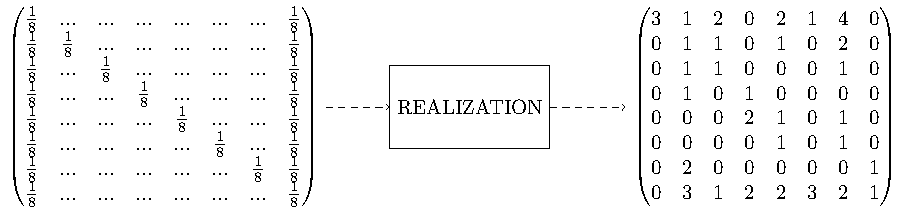
\includegraphics{manuscript_files/figure-latex/tikz-ex-1} \end{center}

In the diagonal, we see how many actors stay in their original
positions. Excluding the diagonal, the column sums capture the amount of
inflow towards a particular position. Conversely, the row sums capture
how many people leave a given location in the landscape. Hence, the
realization matrix allows us to chart the inflows to, and outflows from,
a particular position.

\hypertarget{adjudicating-between-models-of-movement}{%
\subsection{Adjudicating Between Models of
Movement}\label{adjudicating-between-models-of-movement}}

Of course, we can only observe the realized transitions in the empirical
context. How can we know the underlying generative model? We can exploit
the fact that certain realization matrices will be more compatible with
some transition matrices than others. One straightforward procedure to
do this is to compare multiple models using the sum of the absolute
differences between the empirical matrix and the realization matrix
predicted by a given movement model:

\[
\text{Prediction Error} = \sum|E-R|
\]

where \(E\) refers to the empirical matrix while \(R\) refers to the
realization matrix.

Lower differences would indicate a better fit between the specified
movement model and the observed data. Let's go back to the example
above. Imagine our empirical matrix looks more similar to the
realization matrix from the random model. Say we want to compare two
movement models that might have produced these data. The first is the
totally random model we saw above. The second is perhaps a more specific
one, which we will call \emph{move at most one}. It states that moves
that imply one step or fewer (like staying) have equal probability,
while those that imply longer distances have zero probability. This is
what the transition matrix for this model would look like:

\[
T_{8,8} =
\begin{pmatrix}
\frac{1}{4} & \frac{1}{4} & \frac{1}{4} & 0 & \frac{1}{4} & 0 & 0 & 0  \\
\frac{1}{4} & \frac{1}{4} & 0 & \frac{1}{4} & 0 & \frac{1}{4} & 0 & 0  \\
\frac{1}{4} & 0 & \frac{1}{4} & \frac{1}{4} & 0 & 0 & \frac{1}{4} & 0  \\
0 & \frac{1}{4} & \frac{1}{4} & \frac{1}{4} & 0 & 0 & 0 & \frac{1}{4}  \\
\frac{1}{4} & 0 & 0 & 0 & \frac{1}{4} & \frac{1}{4} & \frac{1}{4} & 0  \\
0 & \frac{1}{4} & 0 & 0 & \frac{1}{4} & \frac{1}{4} & 0 & \frac{1}{4}  \\
0 & 0 & \frac{1}{4} & 0 & \frac{1}{4} & 0 & \frac{1}{4} & \frac{1}{4}  \\
0 & 0 & 0 & \frac{1}{4} & 0 & \frac{1}{4} & \frac{1}{4} & \frac{1}{4} 
\end{pmatrix}
\]

We can compare the empirical matrix with the realization matrices
produced by the proposed models. Given that there is stochasticity
involved in moving from the transition matrix to the realization matrix,
we want to iterate over this process several times to build a reliable
picture of what model of movement is more compatible with the data we
have observed. We can, for instance, compare 100 realization matrices
from each model with our empirical matrix, and then take the median
prediction error. Subsequently, we can iterate over these process
several times to get a distribution of median prediction errors. Figure
2 shows these distribution for our current example:

\begin{figure}[htp]
\begin{center}
\caption*{Figure 2: Adjudication Example}

\begin{center}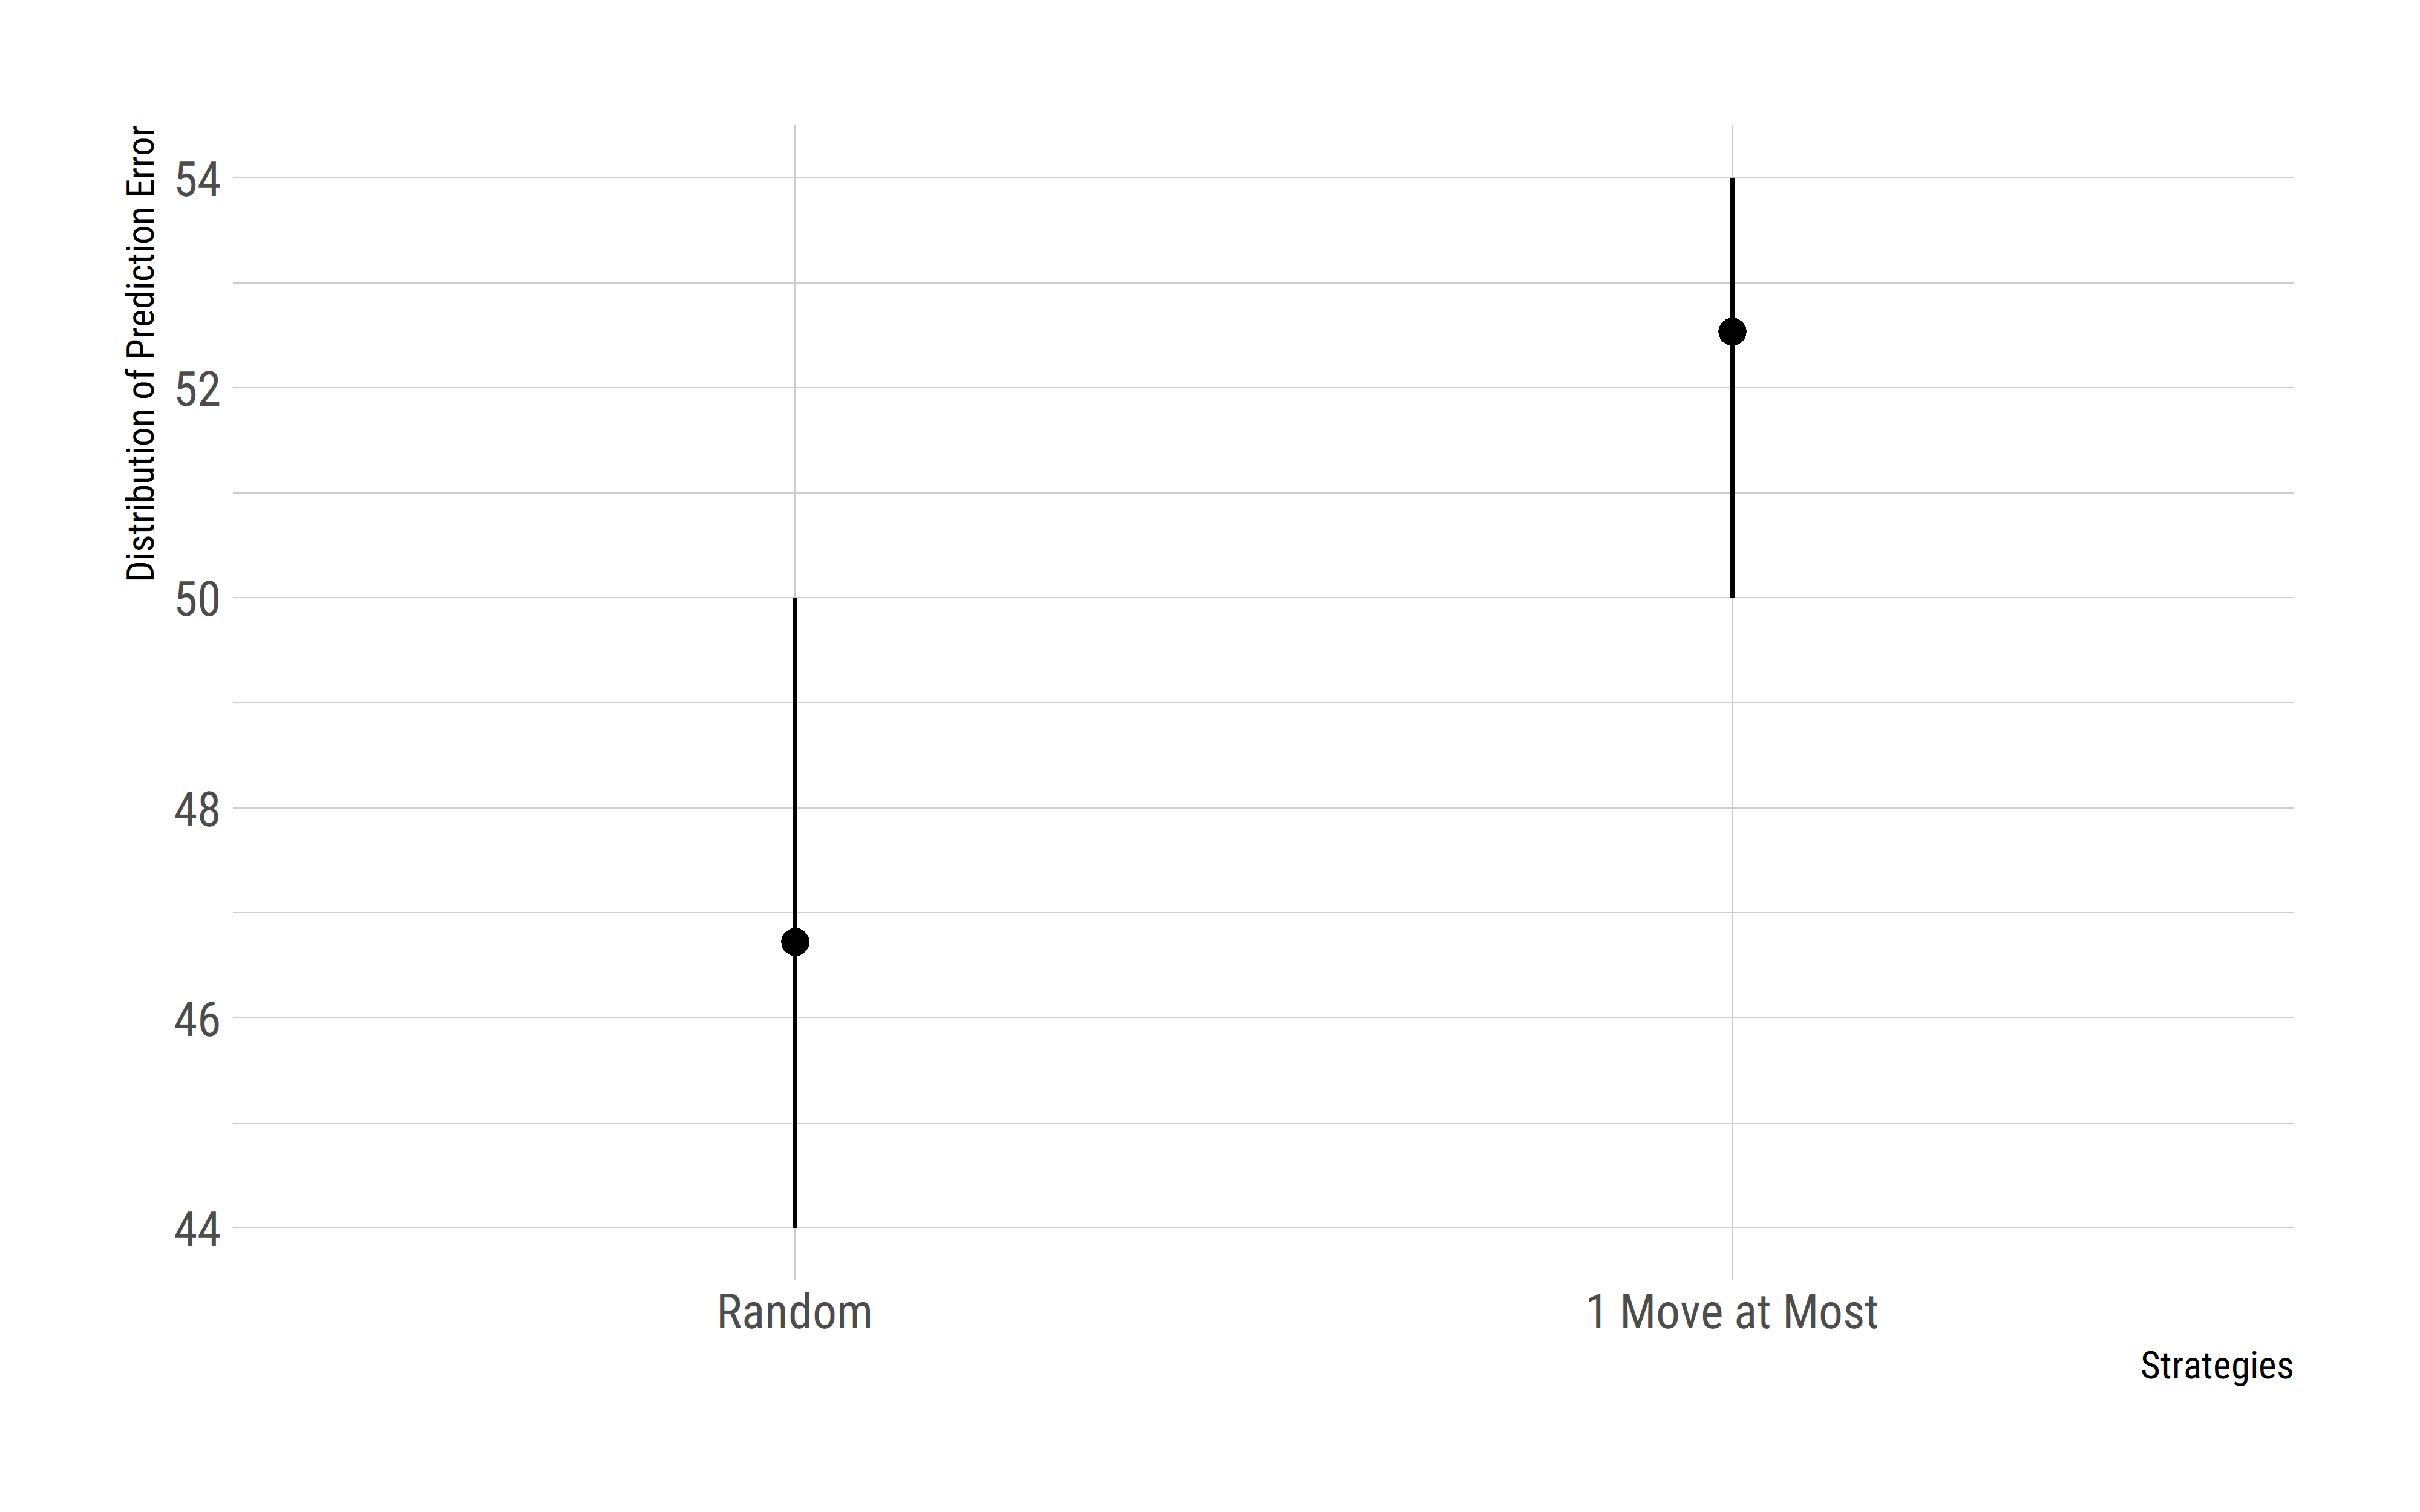
\includegraphics[width=1\linewidth]{../figures/figure_2} \end{center}

\end{center}
\footnotesize{\textit{Notes:} The figure depicts the simulated median prediction errors for two generative models.}
\end{figure}

Here, the points represent the mean prediction error and the lines cover
the range between the 25th and 75th percentiles. We notice that, even
though we have a relatively few agents in our example (\emph{N} = 46),
our method favors the movement model that actually reproduced the data.
The differences, however, are not that big, which suggests that our
capacity to tell apart these two different models --conditional on the
observed data-- is limited. Nonetheless, even in this minimal example,
we see that our method has the capacity to adjudicate between two models
of movement, pointing towards the more plausible data-generating
process.

\hypertarget{an-analysis-of-cultural-movement}{%
\section{An Analysis of Cultural
Movement}\label{an-analysis-of-cultural-movement}}

We now turn to our empirical exercise. In this section, we test several
generative models to see the extent to which the structure of a cultural
landscape is predictive of subsequent movement. We do this in four
steps. First, we propose several models of movement that we derived from
theoretical expectations. We then describe three landscapes that provide
insights into our expectations. Third, we analyze the predictions from
five generative models against the empirical data. In the last step, we
turn to simulation models to explore the implications of these
predictions.

\hypertarget{generative-models-of-cultural-movement}{%
\subsection{Generative Models of Cultural
Movement}\label{generative-models-of-cultural-movement}}

We assess how different models of movement capture the transitions
observed in three landscapes of personal culture. We compare five
models. The first two are models that are either fully agnostic or fully
deterministic: the \emph{random} model and the \emph{always stay} model.
These models do not incorporate any information about the current state
of the landscape or its topology; either all movements are equally
likely or no one moves, regardless of how the landscape is organized. We
also examine three models that consider some information about the
topology of the landscape. The first is \emph{move at most one}, which
assigns equal probability to staying in one's initial position or moving
to one of the adjacent locations. This is a less stringent version of
\emph{always stay}, and it assumes that actors are likely to stay put in
a given region of the cultural landscape. The models that incorporate
the most information about the landscape are the \emph{distance-based}
model and the \emph{gravitational} model. For the former, the
probability of movement to each position is inversely proportional to
the squared distance between positions. The latter is similar, but it
incorporates the topology of the landscape fully: simply, the
probability of moving to a position is proportional to the current
occupancy of that position divided by the squared distance from the
current location.

The set of generative movement models we examine is based on current
work on change and stability in personal culture (Kiley and Vaisey 2020;
Lersch 2023; Vaisey and Lizardo 2016). These studies state that, while
the current occupancy of positions is a reliable predictor of whether
actors will stay there, there is ample evidence of random and erratic
movement as well. Therefore, the \emph{always stay} and \emph{random}
models are extreme and highly implausible abstractions of these
findings. That being said, the relative accuracy of these models of
movement should tell us something about which one of these two processes
--stasis or randomness-- is more informative about a given landscape.
The other models add further assumptions: move at most one is derived
from Kiley's (2023) work, which shows that, when respondents move, they
tend to stay put within particular regions of the cultural landscape.
The distance-based model is a more explicit way of modeling this
process, making it so that long-distance transitions are not impossible
but increasingly more unlikely. Finally, the gravitational model of
movement combines several ideas. It emphasizes the notion of conformity
-- that more populous positions are both more likely to keep their
current occupants and to attract newcomers (Falandays and Smaldino 2021;
Parsons 1951). However, it also captures the idea that the distance
between positions mediates this process. In other words, a move to a new
position, regardless of how well populated it currently is, becomes less
likely if such a move would entail traversing long distances across the
cultural landscape.

\hypertarget{data-and-analytic-strategy}{%
\subsection{Data and Analytic
Strategy}\label{data-and-analytic-strategy}}

To adjudicate the relative explanatory power of these generative models,
we use survey data from the National Study of Youth and Religion (NSYR),
a longitudinal and nationally representative survey of adolescents and
early adults in the United States. The first wave of the NSYR was
fielded in 2002 and 2003 with 3,370 respondents aged 13 to 17. In
approximately two-year intervals, the NSYR conducted three subsequent
surveys (2005, 2007-2018, and 2012-2013), which allows us to follow the
trajectories of personal culture among adolescents and early adults -- a
demographic that tends to display some durable change (Guhin, Calarco,
and Miller-Idriss 2021; Keskintürk 2022; Kiley and Vaisey 2020).
Moreover, the questions touch on a wide array of subjects, from religion
to abstract questions about morality. This allows us to build different
cultural landscapes with varying topographies, and examine how agents
move across them.\footnote{Since most of these questions had been
  included as of Wave 2, we use Waves 2, 3, and 4 in the upcoming
  analyses. To mitigate confusion, we refer to these waves as Time 1,
  Time 2, and Time 3.}

We analyze movement across three landscapes with widely different
features. The first is made up of seven questions around religion --
e.g., whether respondents believe in angels, miracles, and the afterlife
(N = 1,684). The second features seven items as well, this time related
to gender and sexuality. These encompass questions about whether mothers
should work or unmarried sex is permissible (N = 1,134). The last
landscape consists of an eclectic set of items with equal length,
ranging from moral relativism to the respondents' belief in God (N =
1,432). Our choice of these landscapes is deliberate: we wanted to build
cultural landscapes that have different topographical features. The
sexuality and gender landscape, for instance, has one highly populated
peak, with other positions only sparsely occupied. This resembles what
scholars of ``rugged landscapes'' call a \emph{mount Fuji} terrain: a
landscape dominated by one global peak. The religion landscape, in turn,
has two highly populated yet distant peaks. Finally, the eclectic
terrain is quite disorganized, lacking clear peaks. Thus, the latter is
the most rugged of the three. Table 1 documents the full set of items.

\begin{table}[!h]

\caption{\label{tab:unnamed-chunk-1}The Items Used for the Analyses}
\centering
\resizebox{\linewidth}{!}{
\fontsize{11}{13}\selectfont
\begin{tabu} to \linewidth {>{\raggedright\arraybackslash}p{5cm}>{\raggedright\arraybackslash}p{2cm}>{\raggedright}X}
\toprule
Landscape & Item & Label\\
\midrule
\addlinespace[0.3em]
\multicolumn{3}{l}{\textbf{Landscape 1}}\\
\hspace{1em}Religion & aftrlife & Belief in Afterlife\\
\hspace{1em}Religion & angels & Belief in Angels\\
\hspace{1em}Religion & astrolgy & Belief in Astrology\\
\hspace{1em}Religion & demons & Belief in Demons\\
\hspace{1em}Religion & god & Belief in God\\
\hspace{1em}Religion & miracles & Belief in Miracles\\
\hspace{1em}Religion & reincar & Belief in Reincarnation\\
\addlinespace[0.3em]
\multicolumn{3}{l}{\textbf{Landscape 2}}\\
\hspace{1em}Gender and Sexuality & abstain1 & Waiting for Sex Until Marriage\\
\hspace{1em}Gender and Sexuality & divrceok & Couples Should Stick to Marriage\\
\hspace{1em}Gender and Sexuality & mandecid & Man Make Important Decisions\\
\hspace{1em}Gender and Sexuality & menwrk & Man Earns the Living\\
\hspace{1em}Gender and Sexuality & unmarsex & Unmarried People Having Sex\\
\hspace{1em}Gender and Sexuality & wommar & Women's Life Without Marriage\\
\hspace{1em}Gender and Sexuality & wrkngmom & A Working Mom's Relationship with Child\\
\addlinespace[0.3em]
\multicolumn{3}{l}{\textbf{Landscape 3}}\\
\hspace{1em}Eclectic & god & Belief in God\\
\hspace{1em}Eclectic & spiritua & Spiritual But Not Religious\\
\hspace{1em}Eclectic & wrldorig & The Origins of the World\\
\hspace{1em}Eclectic & moralrel & Moral Relativism\\
\hspace{1em}Eclectic & viewrel & The Views About the Truth of Religion\\
\hspace{1em}Eclectic & relprvte & Religion: Private or Public\\
\hspace{1em}Eclectic & okayconv & Converting Others to Religion\\
\bottomrule
\end{tabu}}
\end{table}

We chose these landscapes precisely because we are interested in how the
features of the space might be associated with different patterns of
movement. Our ultimate goal is to try to understand whether the layout
of a given cultural landscape is associated with certain trajectories.
Figure 3 depicts the layout and topography of these cultural landscapes.

\begin{figure}[htp]
\begin{center}
\caption*{Figure 3: Cultural Landscapes}

\begin{center}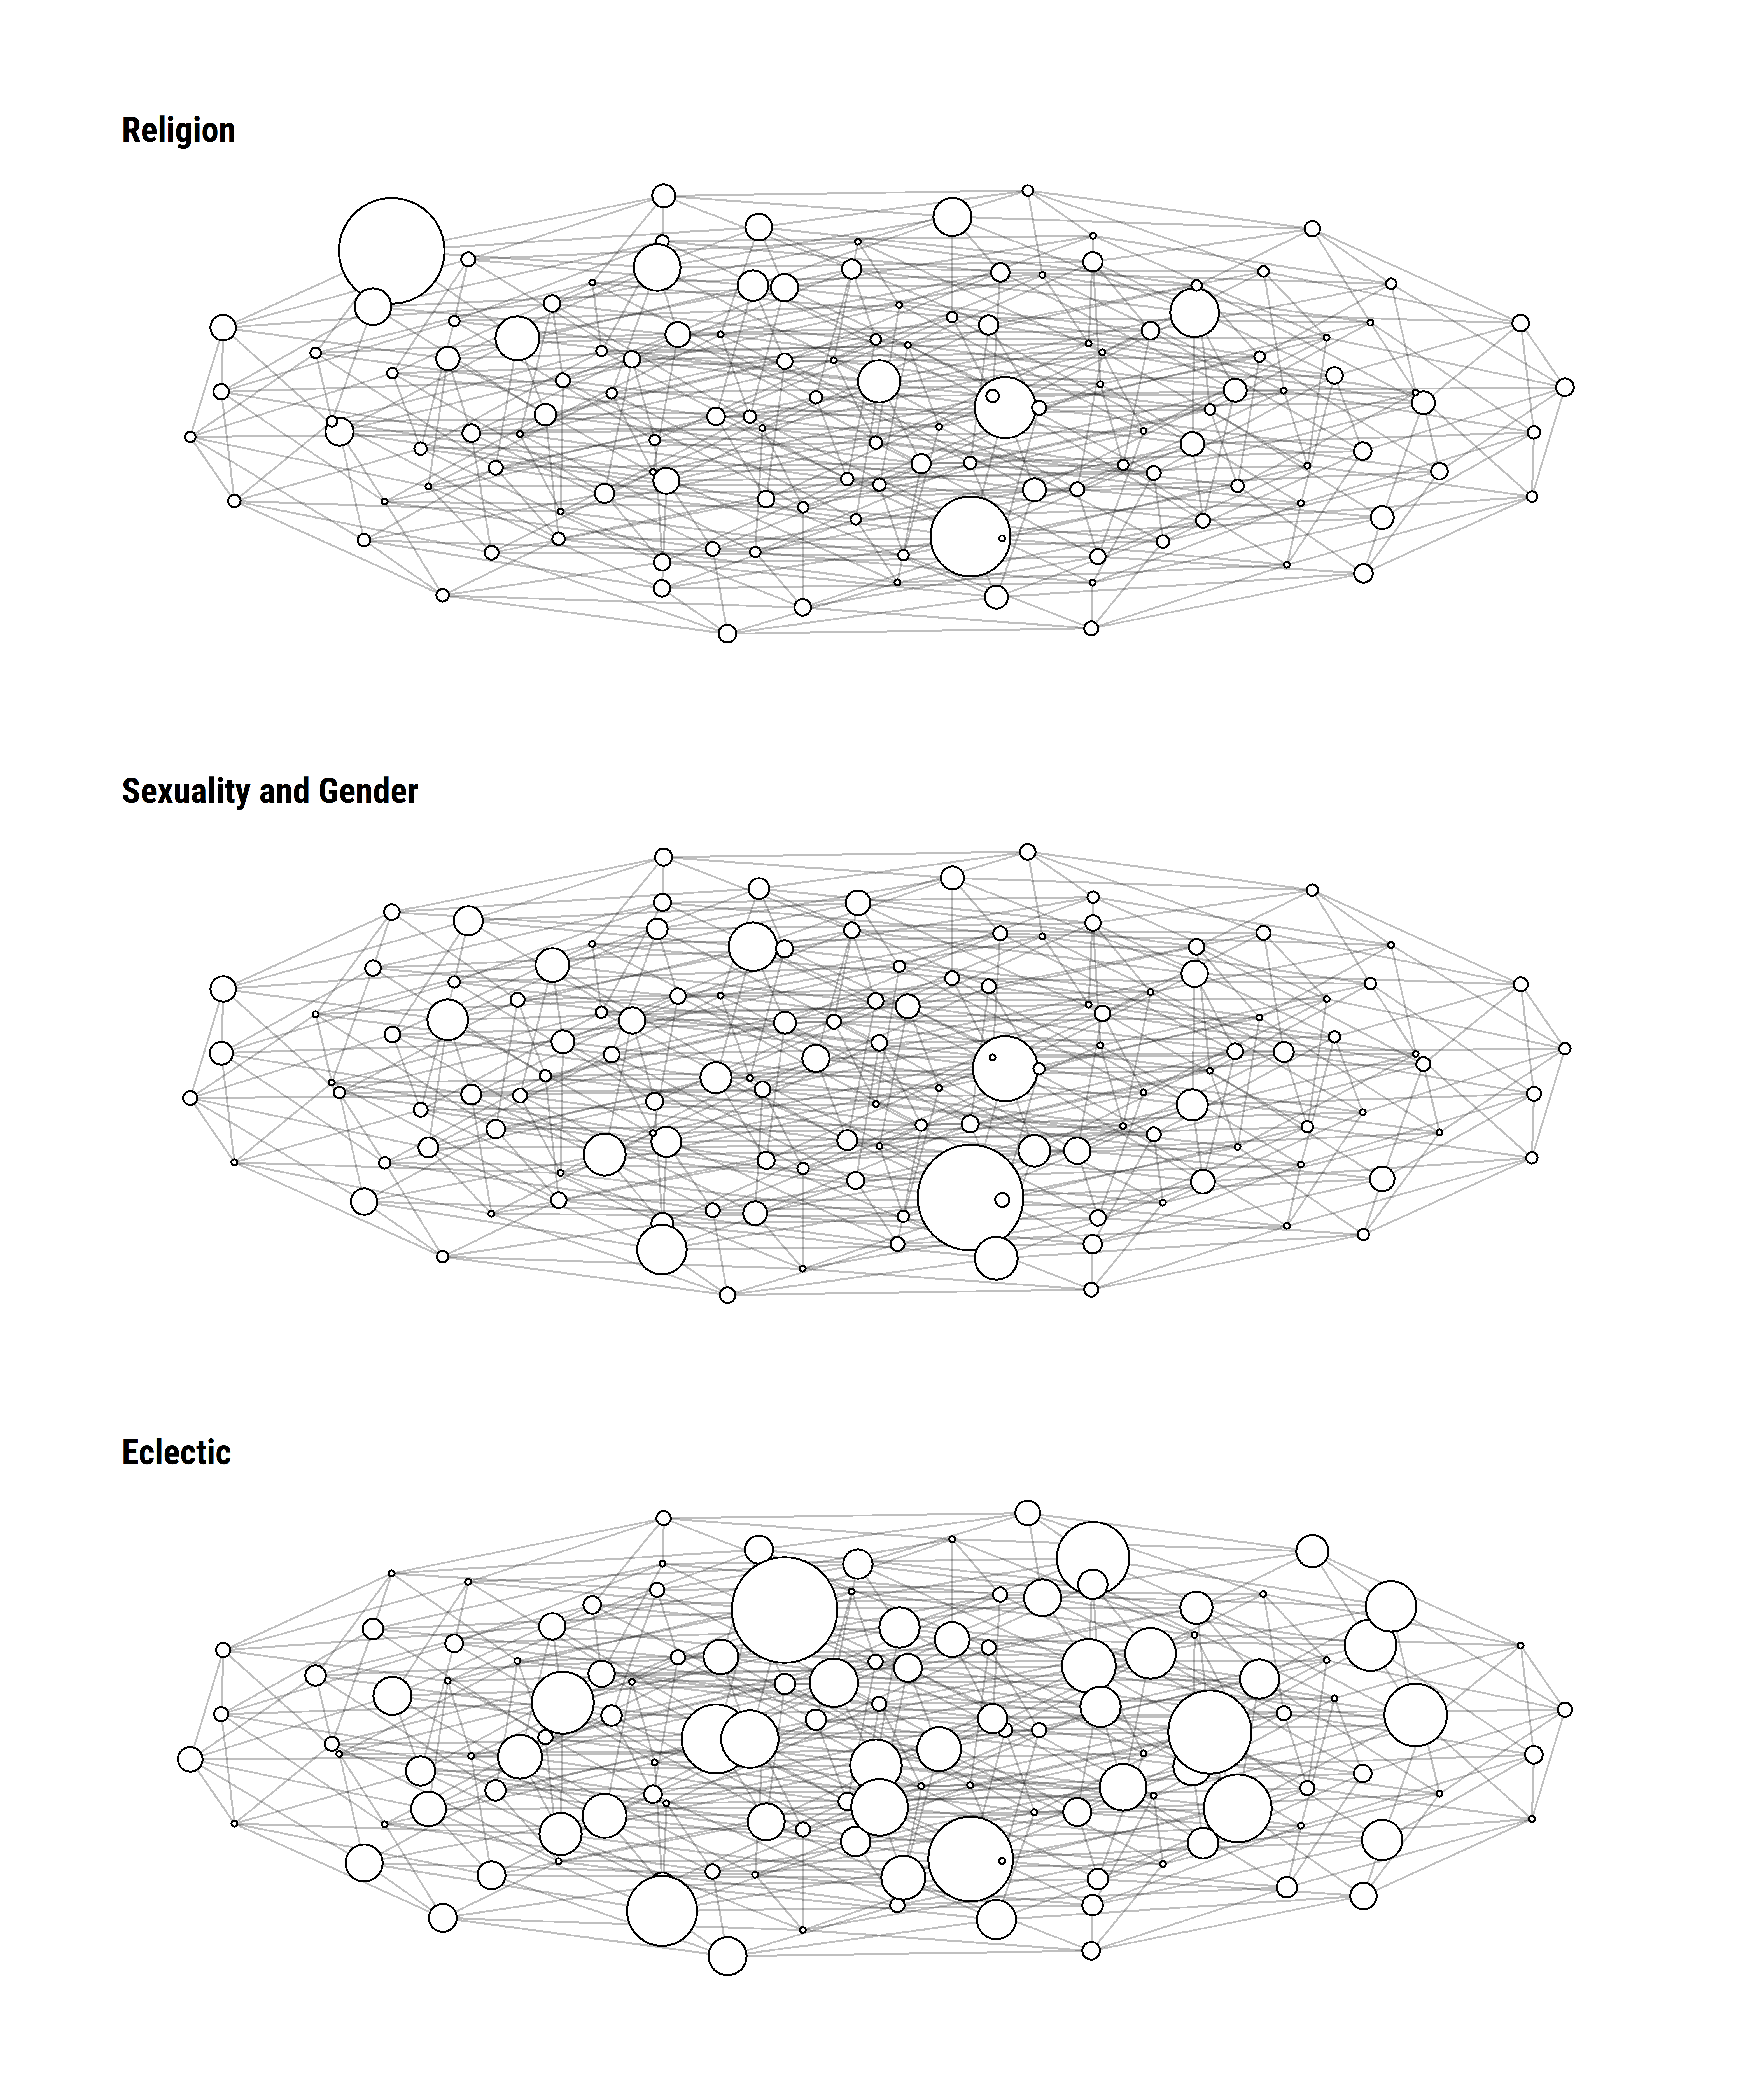
\includegraphics[width=1\linewidth]{../figures/figure_3} \end{center}

\end{center}
\end{figure}

\hypertarget{empirical-results}{%
\subsection{Empirical Results}\label{empirical-results}}

For each of the three cultural landscapes, we examine the relative
explanatory power of the five movement models outlined above. In other
words, we assess how likely each model --with their respective
transition matrices-- is to have generated the transitions we see in our
empirical data. Figure 4 depicts the distribution of prediction errors
for each movement model for each landscape.

\begin{figure}[htp]
\begin{center}
\caption*{Figure 4: Prediction Errors from Empirical Models}

\begin{center}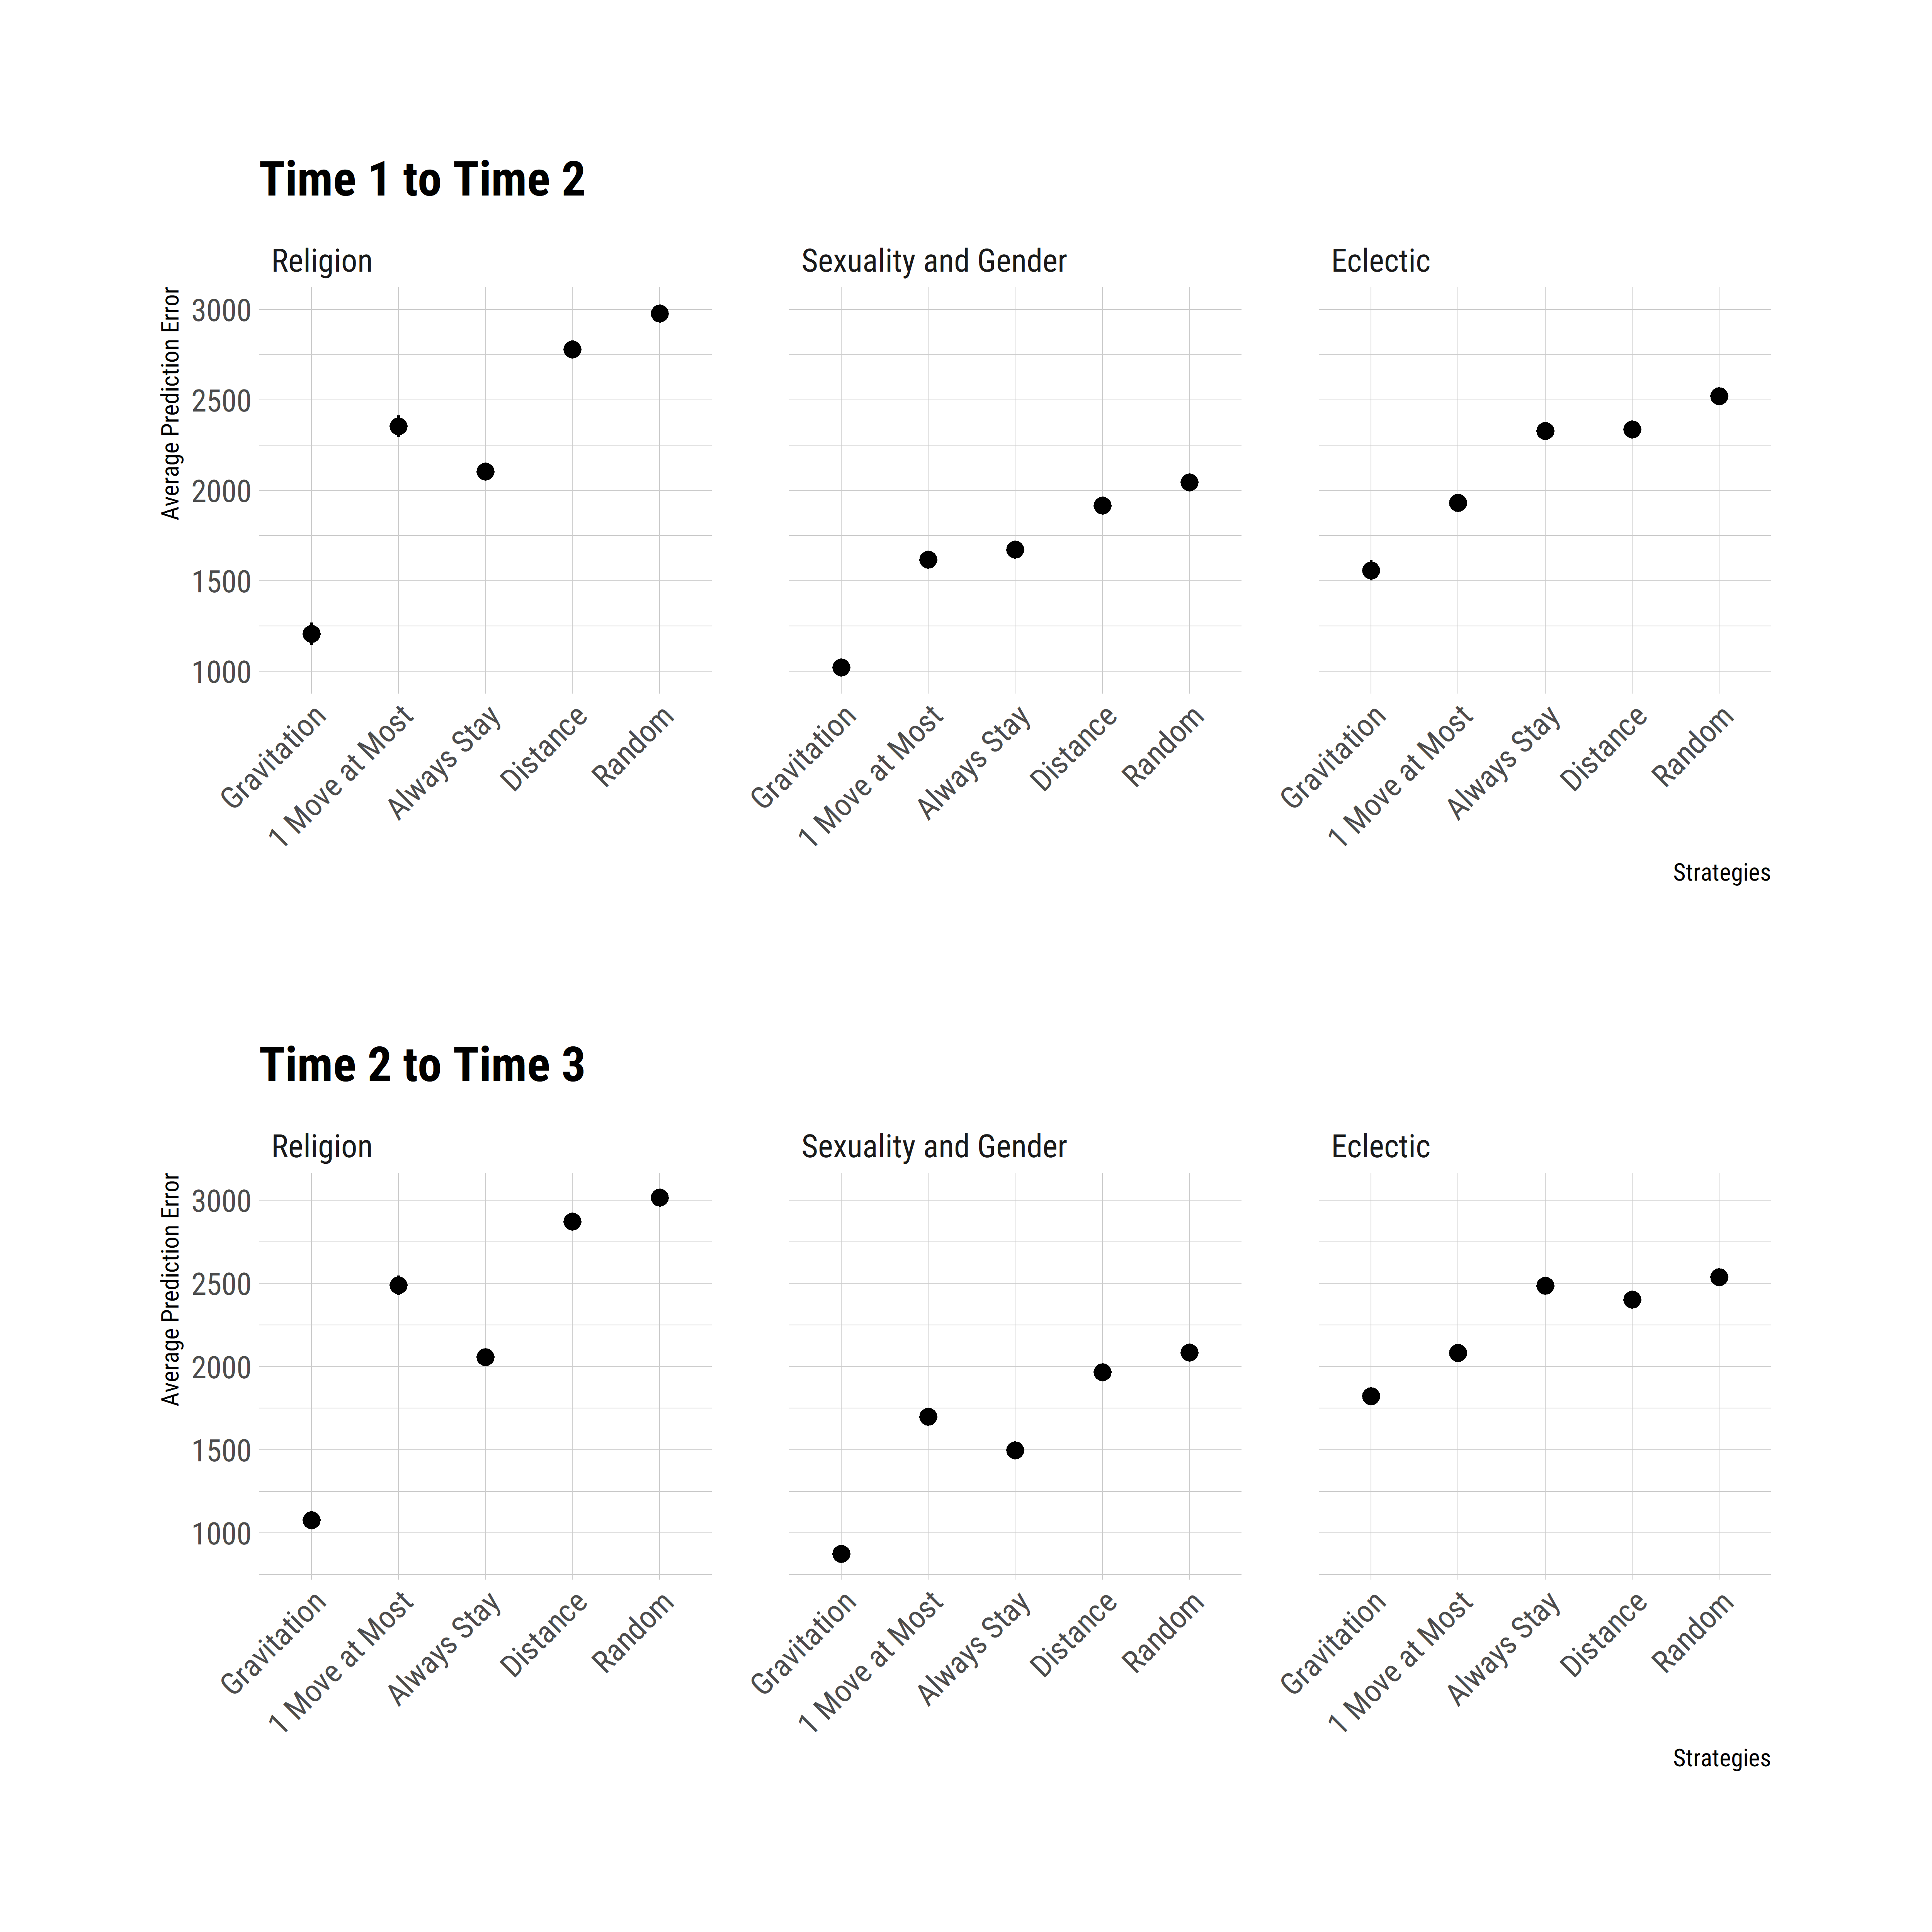
\includegraphics[width=1\linewidth]{../figures/figure_4} \end{center}

\end{center}
\end{figure}

The first general trend we notice is that the gravitational model is the
one that best captures the patterns of movement in the data, across all
landscapes. Second, we see that the random movement and distance-based
models miss the mark the most often. Incidentally, the high inaccuracy
of the latter gives us an indication that knowing the current occupancy
of each position is important for understanding what kind of transitions
people will make.

The greater explanatory power of the gravitational model is perhaps
expected given that it is the model that incorporates the most
information. The gravitational model has more parameters --it takes into
account information about the distance between positions \emph{and} the
current occupancies-- and, therefore, is the most flexible among our
five candidates. Therefore, the gravitational model can make vastly
different predictions depending on the structure of the initial
landscape. It is thus useful to examine the second most informative
model. This is equivalent of asking, ``what other model does the
gravitational model most resemble in a given landscape?''

We see that the gravitational model seems to have a different
relationship with the other models, and this varies across landscapes.
In the Religion landscape, we find that the second most explanatory
model is \emph{Always Stay}. This hints at the fact that stasis is a
dominant pattern in this system: most people are staying in their
original positions. This gives us an additional sense that gravitation
can in fact predict stasis: it would be the most likely outcome in a
system where there are highly occupied positions away from each other.
Their gravitational pull is nullified by distance and by the
countervailing forces of other attractors -- stasis, then, is the
compromise. As we mentioned above, this is precisely the topography of
the Religion landscape.

For the Sexuality and Gender and the Eclectic landscapes, we see that
the \emph{Move One at Most} is the second most appropriate model. This
means that gravitation is predicting either stability or small movements
around the original position. However, note the relationship between
\emph{Move One at Most} and \emph{Always Stay} in each landscape. For
the Sexuality and Gender, both models are quite close in their
prediction errors. This means that, while there are short-distance
transitions, stasis is also a common pattern. For the Eclectic
landscape, in turn, these models have quite different explanatory
powers. This means that gravitation here does really predict
considerable movement, and betting that people will stay in their
original position is not as reliable.

Our central finding is that the gravitational model is the most
predictive, but this model implies different patterns of movement
depending on the layout and topography of the initial landscape. Knowing
the current organization of a landscape --the distance between positions
and how these are occupied-- is thus highly useful for predicting how
agents will move. But the kind of patterns of movement we expect depends
on the organization of the landscape itself.

\hypertarget{simulation-studies}{%
\subsection{Simulation Studies}\label{simulation-studies}}

To further reinforce this argument, we can examine simulations where we
start with the initial organization of each of our landscapes
constructed using the NSYR and let the system develop according to a
gravitational model of movement. Figure 5 provides one such simulated
development: we simulate data as if it was produced by a gravitational
model, and examine the explanatory power of each of our five models. For
these simulations, we run 100 iterations and take the median prediction
error. Then, we repeat this process 50 times.

\begin{figure}[htp]
\begin{center}
\caption*{Figure 5: Prediction Errors from Simulated Models}

\begin{center}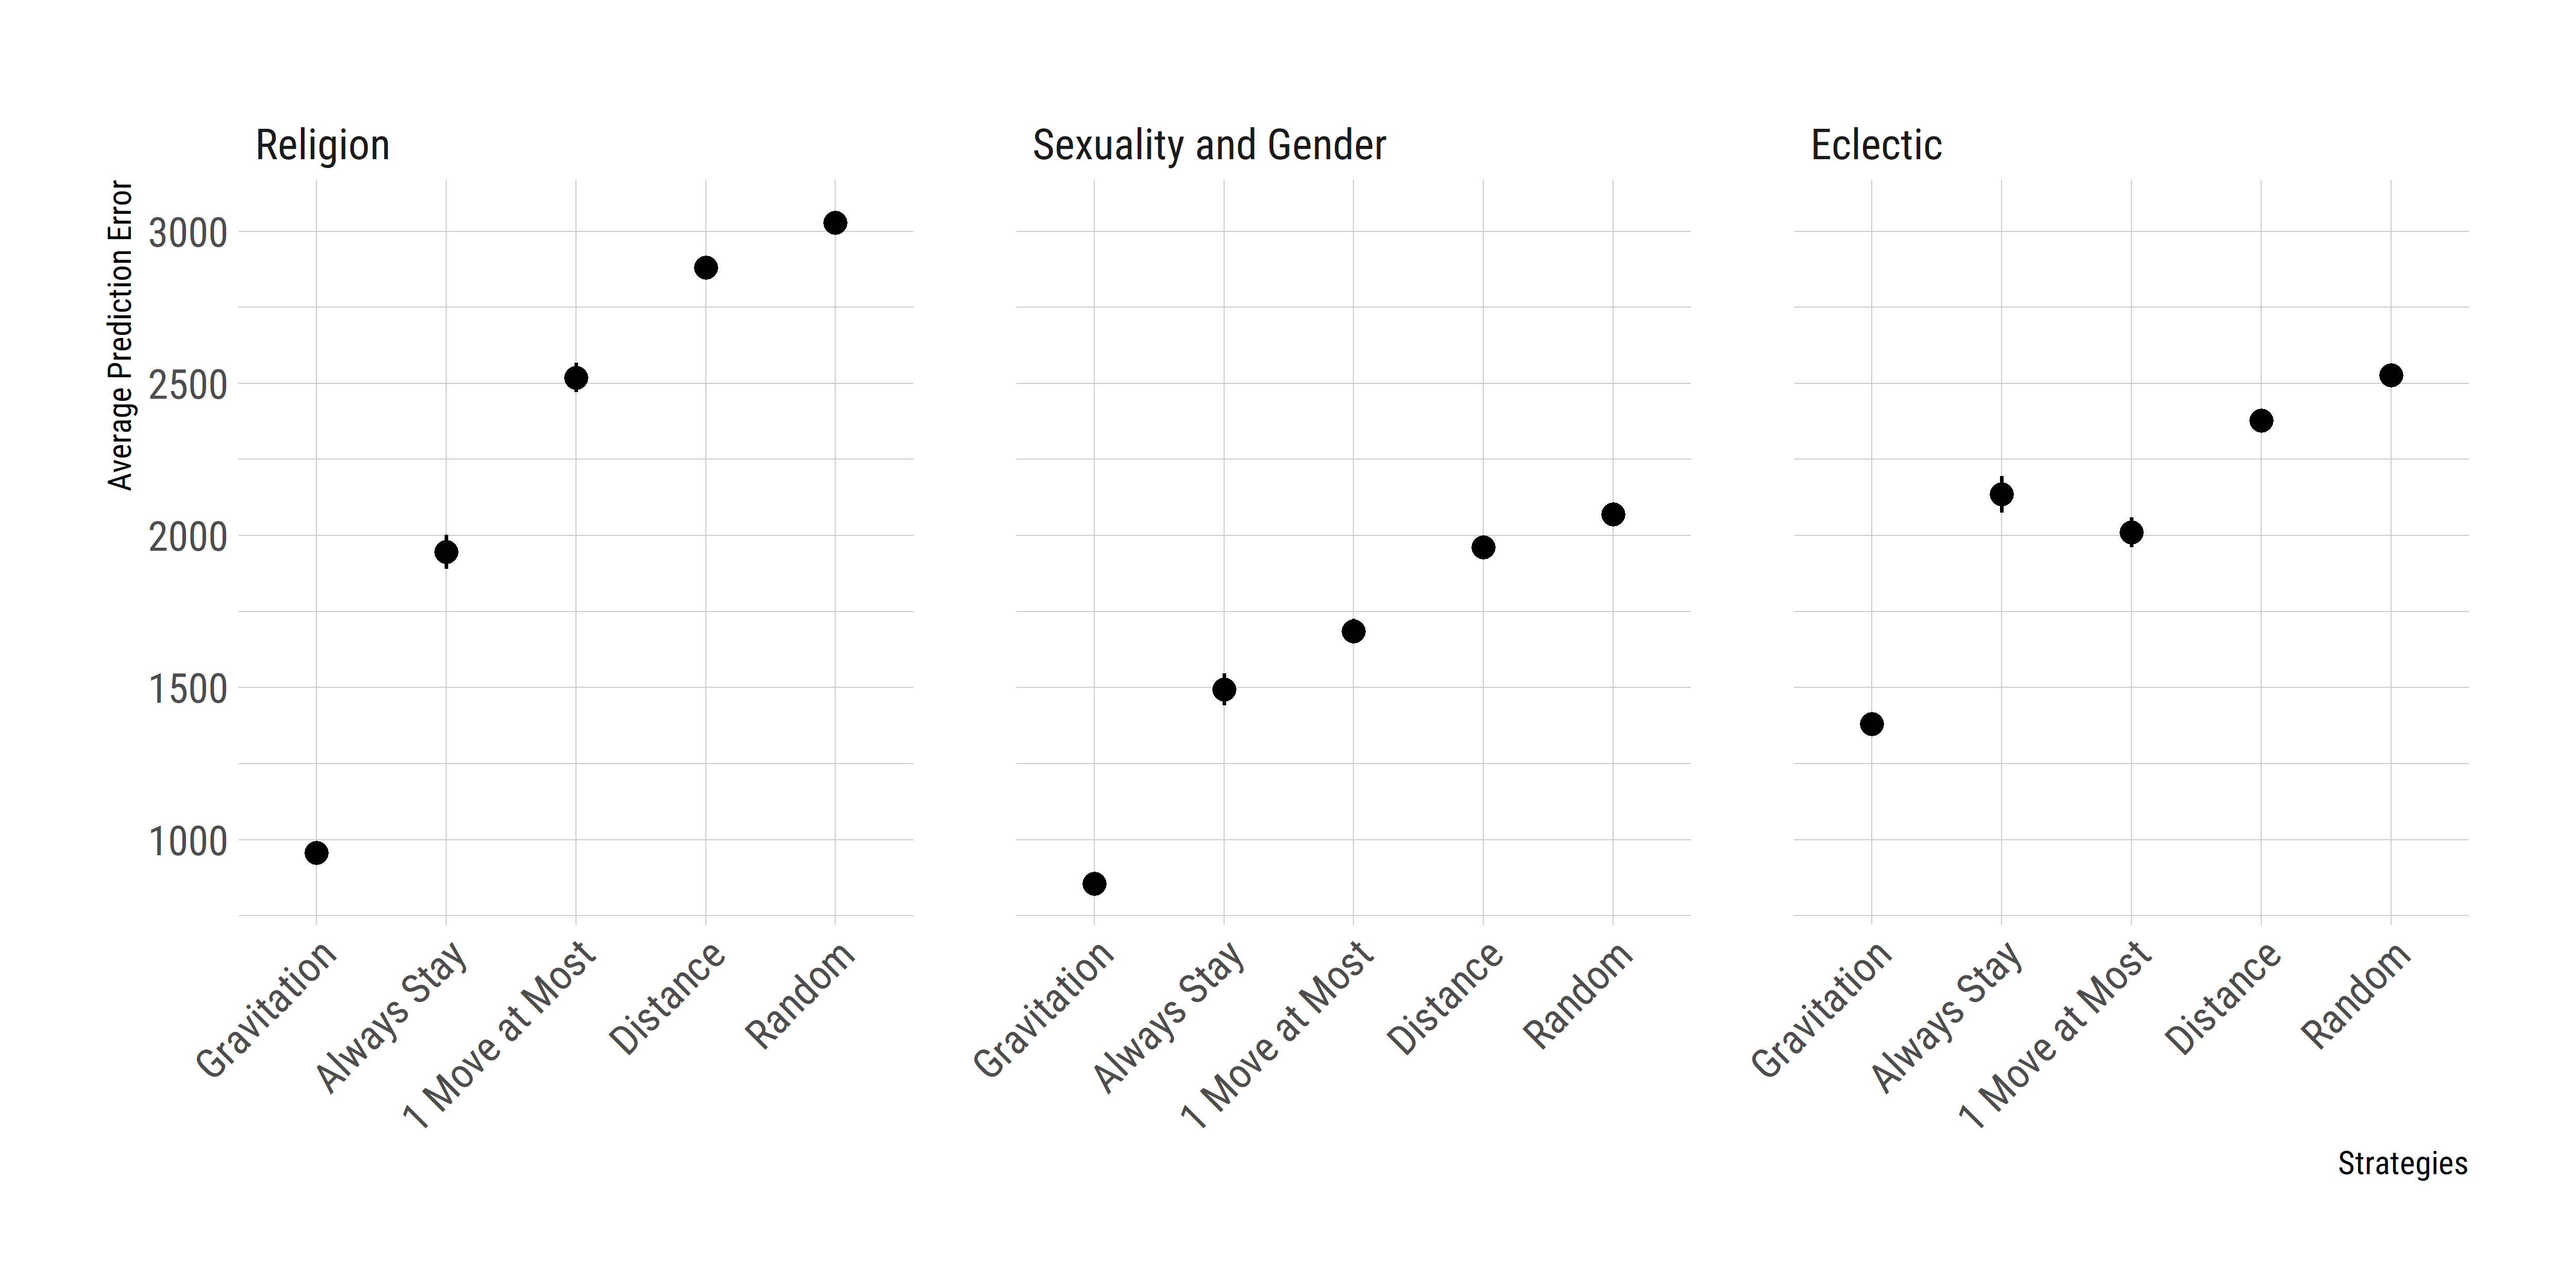
\includegraphics[width=1\linewidth]{../figures/figure_5} \end{center}

\end{center}
\end{figure}

Again, we see similar patterns, suggesting that, even if the
gravitational model is the ``true'' data generating process of these
transitions, we should expect to see different patterns of movement in
each landscape. In a landscape dominated by one peak, like the Sexuality
and Gender landscape, we should expect to see a lot of people staying at
that peak, but also some inflow towards that global attractor.
Gravitation, then, resembles a combination of \emph{Always Stay} and
\emph{Move at Most One}. In a landscape with a few peaks that are far
apart, like the Religion one, we expect stasis, as these highly
populated and distant peaks retain their population. Gravitation here
looks like \emph{Always Stay}. Finally, in a relatively disorganized and
flat landscape, like our eclectic terrain, we expect more movement,
mostly made up of short-distance transitions.

Notice, however, that there are differences between our empirical and
simulated results. While the overall general trends are similar, there
are points of divergence. For example, in the Sexuality and Gender
landscape, now \emph{Always Stay} is a more adequate model than
\emph{Move at Most One}, though the differences remain small. In turn,
for the Eclectic landscape, the difference in accuracy between
\emph{Move at Most One} and \emph{Always Stay} is reduced. This
differences imply that the gravitational model --while adequate-- is not
capturing all the trajectories in the empirical data. This is
unsurprising; we should not expect any model to capture all the patterns
in the data. But the specific ways in which models fail can be
informative. In general, it seems like in the empirical data we are
seeing more stasis than the purely gravitational model would predict.

An important implication of this exercise is that the layout of the
landscape not only affords certain patterns of movement, but also a
certain level of \emph{overall} movement. Figure 6 shows the percentage
of agents that moved in our simulations for each of the landscapes.

\begin{figure}[htp]
\begin{center}
\caption*{Figure 6: The Percent of Changers in Simulated Results}

\begin{center}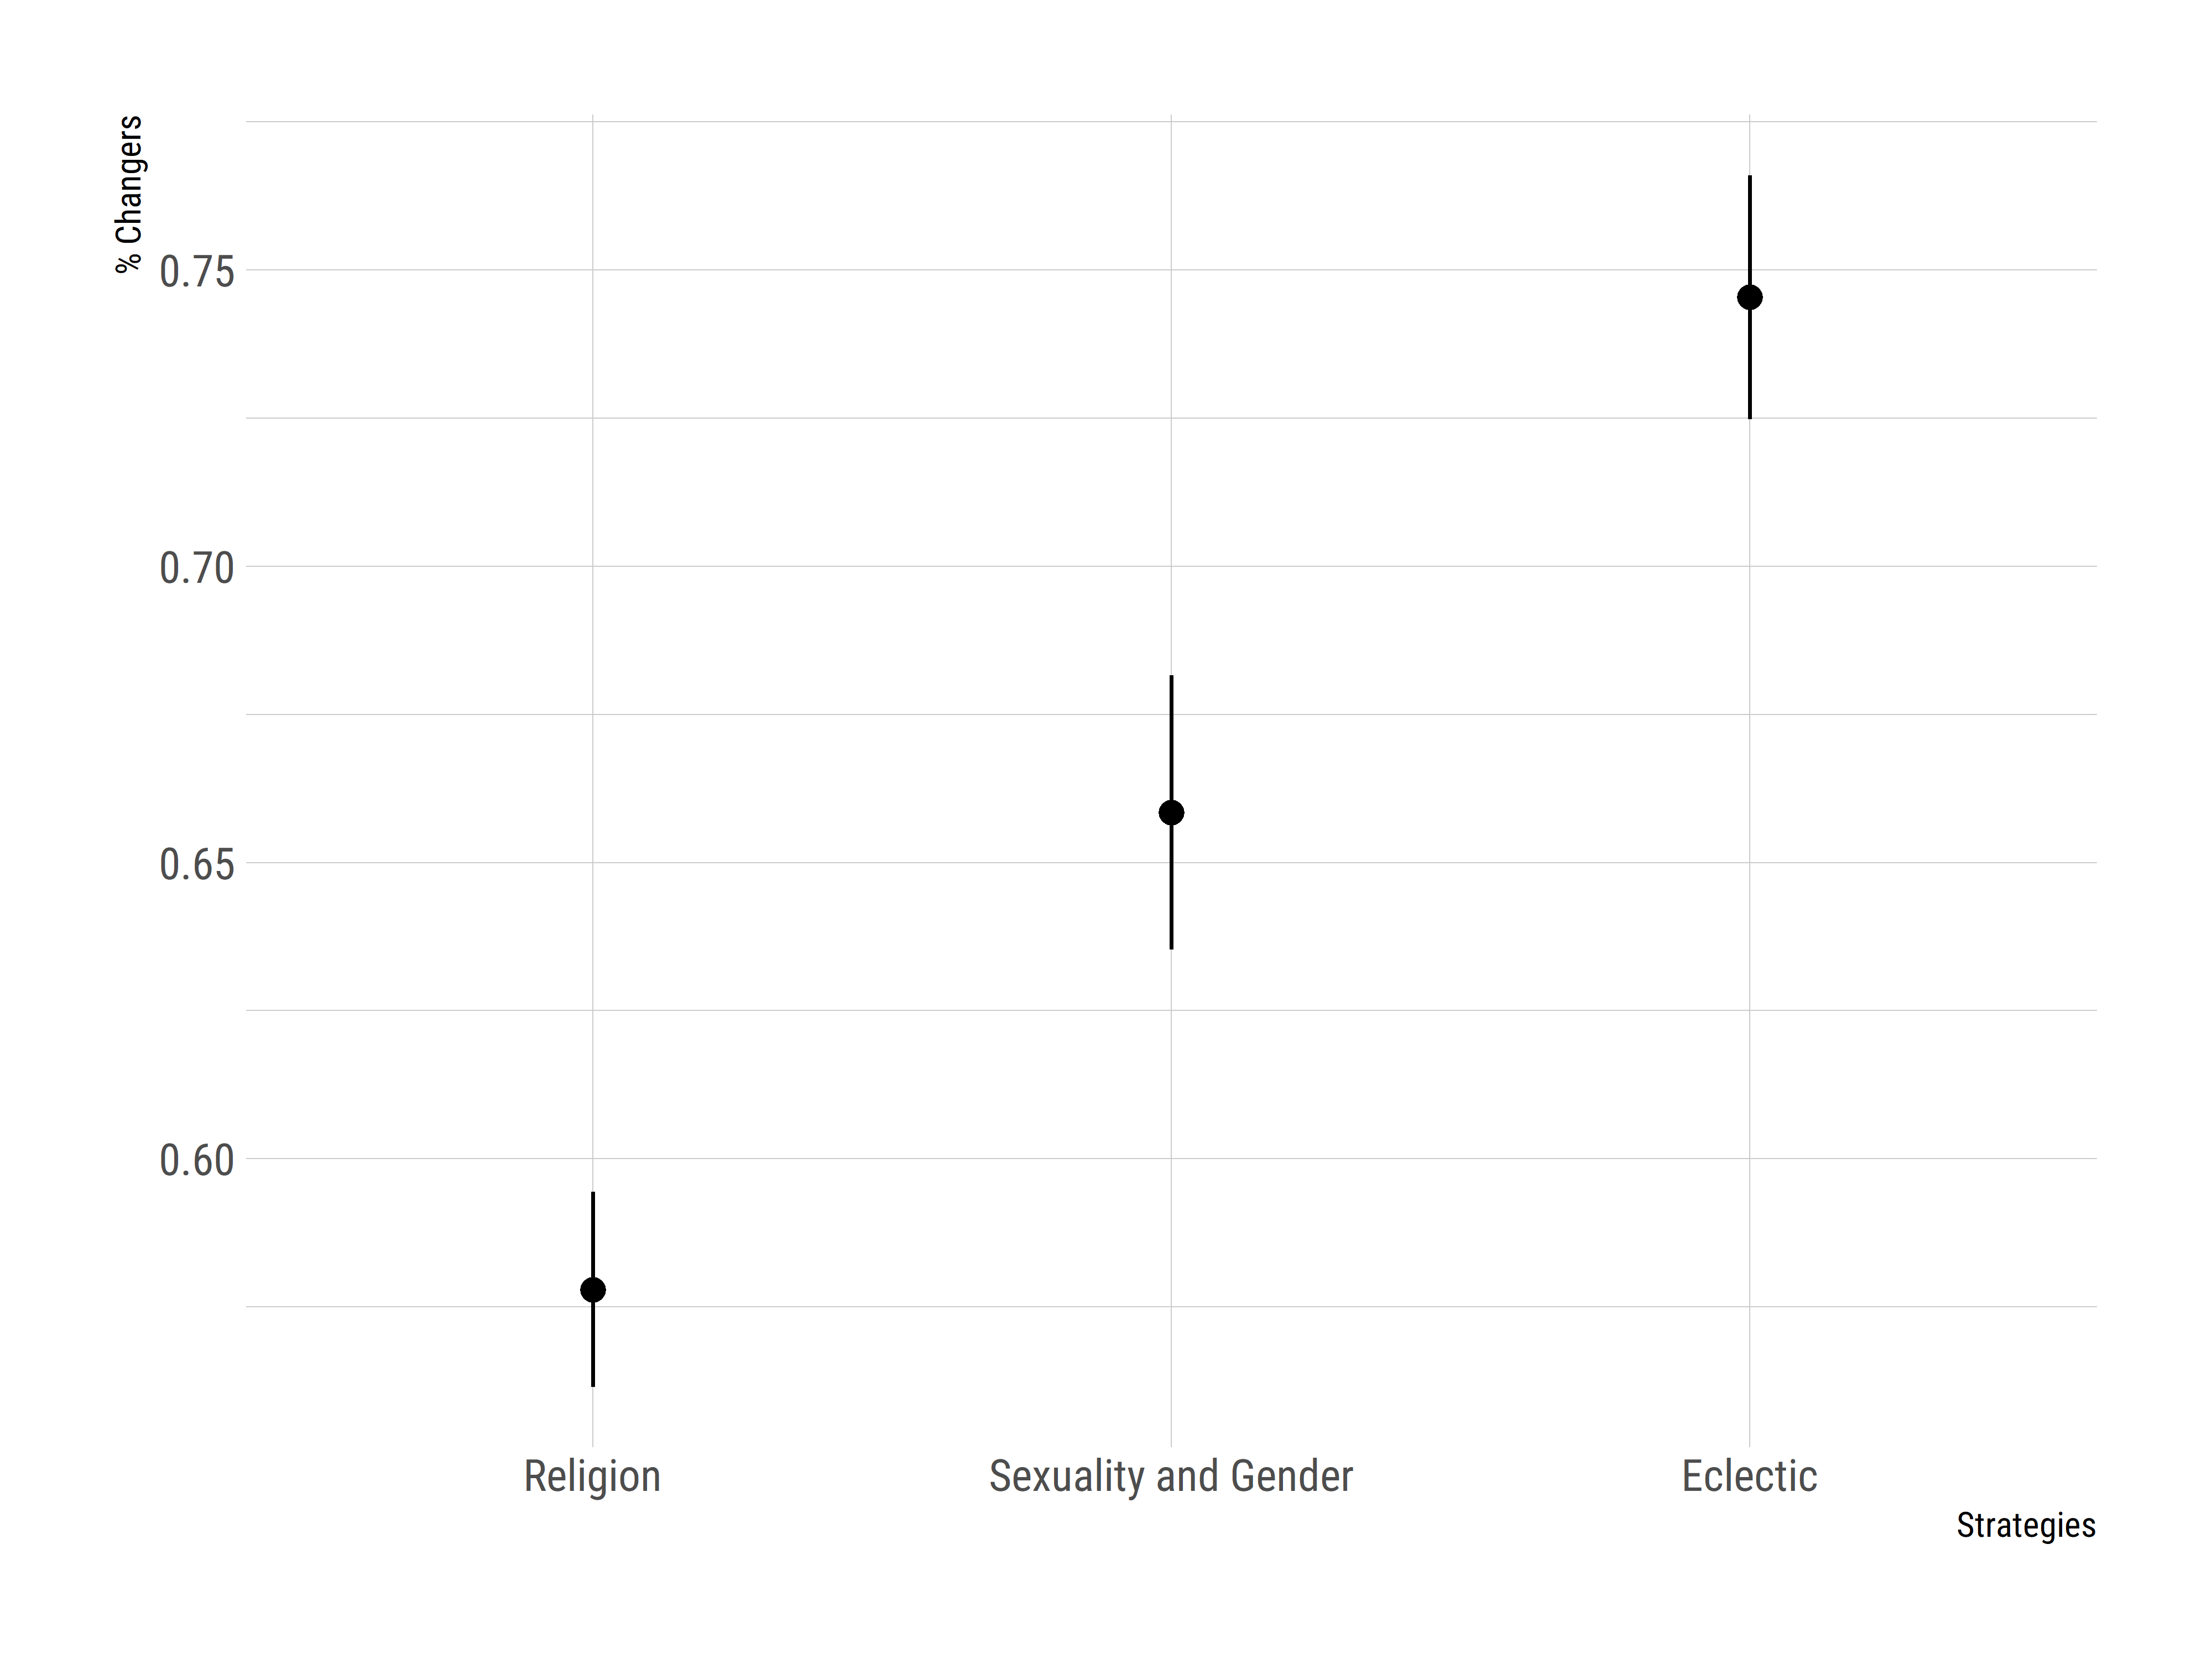
\includegraphics[width=1\linewidth]{../figures/figure_6} \end{center}

\end{center}
\end{figure}

Again, we notice that the multi-polar landscape, like the Religion one,
experiences the least amount of movement. It is followed by the
single-peak landscape, where there is stasis but also considerable
inflow towards the global high point. Lastly, the most rugged landscape
also exhibits the highest proportion of overall movement. The
topography, then, gives us information about the transitions and the
overall proportion of movement we should expect in a landscape.

\hypertarget{discussion}{%
\section{Discussion}\label{discussion}}

In this article, we argue that the common metaphor of culture as a
landscape is not only useful for understanding how culture is organized
--i.e., as a cartographic exercise-- but also for analyzing how people
move across cultural positions. We note that different disciplinary
efforts have converged in certain algebraic representations of cultural
landscapes, where binary strings represent the presence or absence of a
certain set of elements that define the positions of the landscape.
These landscapes have two central features: cardinality and topography.
The former refers to our ability to enumerate the positions that
constitute a space and to know how close or far they are from each
other. The latter, in turn, is concerned with features of the positions
themselves, like how efficacious they are or --in our case-- how
well-populated they are. Echoing Martin (2000), we contend that
capturing the layout of these landscapes is also helpful for
understanding how people will move across them.

To test this idea, we examined trajectories of cultural movement in the
NSYR. We argued that understanding movement across landscapes of
personal culture can be captured by a Markovian process where each
position in the landscape is associated with a set of transition
probabilities. By varying these transition probabilities, it is possible
to build generative models of movement that are explicit about the kind
of trajectories we expect to see in a given landscape. We then compared
the predictions made by different generative models with the observed
empirical data in order to adjudicate their explanatory power. We found
that a gravitational model --one that calculates transition
probabilities according to the occupancy of positions and the distance
between them-- is the most adequate model for explaining the observed
trajectories.

However, we found that the kind of trajectories that such a
gravitational model would predict depend heavily on the initial layout
of the landscape. This is the central insight of our analysis. Both in
our empirical analyses and simulations, we saw that the organization of
the landscapes is informative for understanding the patterns of movement
that we should expect to see. In general, we noticed that the
``ruggedness'' of the landscape is particularly relevant. In the
eclectic landscape, for instance, we noticed a high proportion of
movement, consisting mostly of short transitions. The Sexuality and
Gender landscape, with its one global peak, exhibited a lot of stasis
but also many agents moving towards that main attractor. The Religion
landscape, in turn, had two peaks that effectively nullified each other,
resulting in a higher proportion of individuals staying in their
original positions. Hence, our analyses suggest that how culture is
organized at one point is instrumental to understanding subsequent
development of culture at the population level.

\hypertarget{the-duality-of-what}{%
\subsection{The Duality of What?}\label{the-duality-of-what}}

One important implication of this study extends to the debates around
the notion of duality in general (Breiger 1974) and the duality of
people and cultural beliefs in particular (Boutyline and Vaisey 2017;
Martin 2000). Sociologists have used the idea of duality to understand
belief systems, cultural schemas, and affiliation networks. Most of
these studies, however, have examined these cultural structures as
\emph{static}. The benefits of this approach notwithstanding,
understanding cultural trajectories requires us to reconceptualize
cultural landscapes as evolving and dynamic set of cultural positions.
This means that relying on one approach or the other --individuals
connected by the pieces of culture they share or cultural elements
linked by the individuals that internalize them-- might provide only a
partial understanding of cultural systems. In fact, the framework of
duality also shapes how we should expect the system to look like in the
future: how agents are distributed across the landscape makes up the
topology of the landscape, while at the same time the topology of the
landscape is informative for understanding how those agents will move.

\hypertarget{the-movement-of-what}{%
\subsection{The Movement of What?}\label{the-movement-of-what}}

Measuring the dynamics of cultural landscapes is quite appealing, though
the price is two strong assumptions. First, the model assumes that the
processes of cultural change and stability depend on the public opinion
field, meaning that the social distribution of ideas is central to
understanding belief dynamics. Yet, two conflicting cultural models can
explain this expectation: it might be that actors learn this structure
early on, and the landscape changes through the replacement of old
actors with the new ones (Vaisey and Lizardo 2016), or certain period
effects might push people to places with high volume through processes
of conformity (DellaPosta et al. 2015). We remain agnostic about either
explanation, though it is important to note that we expect the
distribution of positions has a say in predicting \emph{both} change and
stability over the survey period.

Second, algebraic representations suffer from important measurement
problems. First, the assumption of binary positions is restrictive, as
it often involves arbitrary cutoffs that eliminate the original
variance. Second, the list of the number of elements \(N\) that defines
the dimensions of our space is unlikely to be exhaustive. Third, and
perhaps most importantly, the survey responses can become too volatile
or uncertain to reliably infer one's position in a belief space, given
that measurement error might affect the overall distribution (Alwin
2007; Zaller 1992).

The measurement problem is a trade-off between recovering \emph{true}
states or ensuring that we get the benefits of being able to locate
positions spatially. Sociologists often build latent state models that
associate cultural profiles not to a specific position in the landscape,
but rather to a set of probabilities that produce a given set of
responses (Kiley 2023). This allows us to bypass potential measurement
errors resulting from a number of factors (Alwin and Krosnick 1991;
Ansolabehere, Rodden, and Snyder 2008), as well as ensuring that the
potential movement we observe is not due to errors. This fends off
uncertainty, but comes with several costs. For instance, given that
latent states are defined qualitatively, we cannot understand the
directionality or distance of trajectories. In other words, we do not
know what transitions are large or small, and whether certain latent
states are closer to others. In this sense, our proposal for measuring
cultural landscapes comes with important caveats, though we believe that
the gains might be useful nonetheless.

\hypertarget{moving-forward}{%
\subsection{Moving Forward}\label{moving-forward}}

We argued that culture as landscape comes with two benefits: (a)
understanding culture as a set of evolving and dynamic positions and (b)
the extension of static cultural representations to dynamic models of
movement. This framework, however, extends to multiple units and
relations. First, the same formal representation applies to
organizational ecologies, where the principle of duality dictates, once
again, the dual relationship between organizational actors and
field-specific ties. Understanding how fields organize around specific
features and the resulting topography might help us predict stability
and change in organizational networks. Second, the framework of culture
as landscape is highly instrumental to understanding historical
emergence of cultural attractors, given that new religions, cultural
movements, or political institutions often redefine the given landscape.
This, in turn, facilitates questions around whether certain features
replicate over time, or whether new features start defining multiple
clusters. Finally, culture as landscape allows us to ask cross-cultural
questions as to the structural similarities among different groups,
particularly with regard to the organization of religion, political
ideologies, or moral frameworks. We hope that researchers find this
approach useful in their own work.

\hypertarget{references}{%
\section*{References}\label{references}}
\addcontentsline{toc}{section}{References}

\hypertarget{refs}{}
\begin{CSLReferences}{1}{0}
\leavevmode\vadjust pre{\hypertarget{ref-alwin2007}{}}%
Alwin, Duane F. 2007. \emph{Margins of {Error}: {A} {Study} of
{Reliability} in {Survey} {Measurement}}. Hoboken, N.J.: John Wiley \&
Sons.

\leavevmode\vadjust pre{\hypertarget{ref-alwin1991}{}}%
Alwin, Duane F. and Jon A. Krosnick. 1991. {``The {Reliability} of
{Survey} {Attitude} {Measurement}: {The} {Influence} of {Question} and
{Respondent} {Attributes}.''} \emph{Sociological Methods and Research}
20(1):139--81.

\leavevmode\vadjust pre{\hypertarget{ref-ansolabehere2008}{}}%
Ansolabehere, Stephen, Jonathan Rodden, and James M. Snyder. 2008.
{``The {Strength} of {Issues}: {Using} {Multiple} {Measures} to {Gauge}
{Preference} {Stability}, {Ideological} {Constraint}, and {Issue}
{Voting}.''} \emph{American Political Science Review} 102(2):215--32.

\leavevmode\vadjust pre{\hypertarget{ref-baldassarri2014}{}}%
Baldassarri, Delia and Amir Goldberg. 2014. {``Neither {Ideologues}
{Nor} {Agnostics}: {Alternative} {Voters}' {Belief} {System} in {An}
{Age} of {Partisan} {Politics}.''} \emph{American Journal of Sociology}
120(1):45--95.

\leavevmode\vadjust pre{\hypertarget{ref-bonikowski2016}{}}%
Bonikowski, Bart and Paul DiMaggio. 2016. {``Varieties of {American}
{Popular} {Nationalism}.''} \emph{American Sociological Review}
81(5):949--80.

\leavevmode\vadjust pre{\hypertarget{ref-boutyline2022}{}}%
Boutyline, Andrei. 2022. {``Public {Opinion} {As} {Cognition} in a
{Disorganized} {Field}.''} \emph{Poetics} 95:101710.

\leavevmode\vadjust pre{\hypertarget{ref-bv2017}{}}%
Boutyline, Andrei and Stephen Vaisey. 2017. {``Belief {Network}
{Analysis}: {A} {Relational} {Approach} to {Understanding} the
{Structure} of {Attitudes}.''} \emph{American Journal of Sociology}
122(5):1371--1447.

\leavevmode\vadjust pre{\hypertarget{ref-breiger1974}{}}%
Breiger, Ronald L. 1974. {``The {Duality} of {Persons} and {Groups}.''}
\emph{Social Forces} 53(2):181--90.

\leavevmode\vadjust pre{\hypertarget{ref-dellaposta2015}{}}%
DellaPosta, Daniel, Yongren Shi, and Michael Macy. 2015. {``Why {Do}
{Liberals} {Drink} {Lattes}?''} \emph{American Journal of Sociology}
120(5):1473--1511.

\leavevmode\vadjust pre{\hypertarget{ref-falandays2021}{}}%
Falandays, J. Benjamin and Paul E. Smaldino. 2021. {``The {Emergence} of
{Cultural} {Attractors}: {How} {Dynamic} {Populations} of {Learners}
{Achieve} {Collective} {Cognitive} {Alignment}.''} \emph{Cognitive
Science} 46(8):e13183.

\leavevmode\vadjust pre{\hypertarget{ref-goldberg2011}{}}%
Goldberg, Amir. 2011. {``Mapping {Shared} {Understandings} {Using}
{Relational} {Class} {Analysis}: {The} {Case} of the {Cultural}
{Omnivore} {Reexamined}.''} \emph{American Journal of Sociology}
116(5):1397--1436.

\leavevmode\vadjust pre{\hypertarget{ref-guhin2021}{}}%
Guhin, Jeffrey, Jessica Calarco, and Cynthia Miller-Idriss. 2021.
{``Whatever {Happened} to {Socialization}.''} \emph{Annual Review of
Sociology} 47:109--29.

\leavevmode\vadjust pre{\hypertarget{ref-hunzaker2019}{}}%
Hunzaker, M. B. Fallin and Lauren Valentino. 2019. {``Mapping {Cultural}
{Schemas}: {From} {Theory} to {Method}.''} \emph{American Sociological
Review} 84(5):950--81.

\leavevmode\vadjust pre{\hypertarget{ref-kauffman1989}{}}%
Kauffman, Stuart A. and Edward D. Weinberger. 1989. {``The NK Model of
Rugged Fitness Landscapes and Its Application to Maturation of the
Immune Response.''} \emph{Journal of Theoretical Biology} 141-2:211--45.

\leavevmode\vadjust pre{\hypertarget{ref-keskinturk2022}{}}%
Keskintürk, Turgut. 2022. {``Religious {Belief} {Alignment}: {The}
{Structure} of {Cultural} {Beliefs} from {Adolescence} to {Emerging}
{Adulthood}.''} \emph{Poetics} 90:101591.

\leavevmode\vadjust pre{\hypertarget{ref-kiley2023}{}}%
Kiley, Kevin. 2023. {``Predictably Unpredictable: The Dynamic Constraint
of Cultural Belief Systems.''} \emph{Manuscript in Preparation}.

\leavevmode\vadjust pre{\hypertarget{ref-kiley2020}{}}%
Kiley, Kevin and Stephen Vaisey. 2020. {``Measuring {Stability} and
{Change} in {Personal} {Culture} {Using} {Panel} {Data}.''}
\emph{American Sociological Review} 85(3):477--506.

\leavevmode\vadjust pre{\hypertarget{ref-leemartin2018}{}}%
Lee, Monica and John Levi Martin. 2018. {``Doorway to the {Dharma} of
{Duality}.''} \emph{Poetics} 68:18--30.

\leavevmode\vadjust pre{\hypertarget{ref-lersch2023}{}}%
Lersch, Philipp M. 2023. {``Change in {Personal} {Culture} {Over} the
{Life} {Course}.''} \emph{American Sociological Review} 88(2):252--83.

\leavevmode\vadjust pre{\hypertarget{ref-lizardo2017}{}}%
Lizardo, Omar. 2017. {``Improving {Cultural} {Analysis}: {Considering}
{Personal} {Culture} in Its {Declarative} and {Nondeclarative}
{Modes}.''} \emph{American Sociological Review} 82(1):88--115.

\leavevmode\vadjust pre{\hypertarget{ref-mark1998}{}}%
Mark, Noah. 1998. {``Birds of a {Feather} {Sing} {Together}.''}
\emph{Social Forces} 77(2):453--85.

\leavevmode\vadjust pre{\hypertarget{ref-martin2000}{}}%
Martin, John Levi. 2000. {``The {Relation} of {Aggregate} {Statistics}
on {Beliefs} to {Culture} and {Cognition}.''} \emph{Poetics}
28(1):5--20.

\leavevmode\vadjust pre{\hypertarget{ref-martin2010}{}}%
Martin, John Levi and Matthew Desmond. 2010. {``Political {Position} and
{Social} {Knowledge}.''} \emph{Sociological Forum} 25(1):1--26.

\leavevmode\vadjust pre{\hypertarget{ref-biggods2013}{}}%
Norenzayan, Ara. 2013. \emph{Big {Gods}: {How} {Religion} {Transformed}
{Cooperation} and {Conflict}}. Princeton: Princeton University Press.

\leavevmode\vadjust pre{\hypertarget{ref-parsons1951}{}}%
Parsons, Talcott. 1951. \emph{The {Social} {System}}. New York:
Routledge.

\leavevmode\vadjust pre{\hypertarget{ref-poulsen2023b}{}}%
Poulsen, Victor Møller and Simon DeDeo. 2023a. {``Cognitive Attractors
and the Cultural Evolution of Religion.''} \emph{Proceedings of the
Annual Meeting of the Cognitive Science Society} 45:3418--23.

\leavevmode\vadjust pre{\hypertarget{ref-poulsen2023a}{}}%
Poulsen, Victor Møller and Simon DeDeo. 2023b. {``Inferring Cultural
Landscapes with the Inverse Ising Model.''} \emph{Entropy} 25(2):264.

\leavevmode\vadjust pre{\hypertarget{ref-vaisey2016}{}}%
Vaisey, Stephen and Omar Lizardo. 2016. {``Cultural {Fragmentation} or
{Acquired} {Dispositions}? {A} {New} {Approach} to {Accounting} for
{Patterns} of {Cultural} {Change}.''} \emph{Socius: Sociological
Research for a Dynamic World} 2:1--15.

\leavevmode\vadjust pre{\hypertarget{ref-wiley1999}{}}%
Wiley, James A. and John Levi Martin. 1999. {``Algebraic
{Representations} of {Beliefs} and {Attitudes}: {Partial} {Order}
{Models} for {Item} {Responses}.''} \emph{Sociological Methodology}
29(1):113--46.

\leavevmode\vadjust pre{\hypertarget{ref-zaller1992}{}}%
Zaller, John R. 1992. \emph{The {Nature} and {Origins} of {Mass}
{Opinion}}. Cambridge: Cambridge University Press.

\end{CSLReferences}

\end{document}
